%%%%%%%% ICML submission version %%%%%%%%%%%%%%%%%
% Content is shared with pre.tex (preprint, Tencent Hunyuan template) through sections/*.tex.
% Numbers, tables and data figures are generated from the frozen data by
%   python3 code/specsched/paper_assets.py <project root> <this folder>
% Uses the ICML 2026 style files; replace icml2026.sty/.bst when the ICML 2027 files are released.

\documentclass{article}
\PassOptionsToPackage{table}{xcolor}
\usepackage{hyperref}
\newcommand{\theHalgorithm}{\arabic{algorithm}}

% blind submission (authors are hidden automatically)
\usepackage{icml2026}
% preprint:      \usepackage[preprint]{icml2026}
% camera-ready:  \usepackage[accepted]{icml2026}

% Shared preamble for example_paper.tex (ICML) and pre.tex (Tencent template).
% Load after the template style. xcolor must already carry the [table] option (\PassOptionsToPackage before the style).
\usepackage{microtype}
\usepackage{graphicx}
\usepackage{booktabs}
\usepackage{tabularx}
\usepackage{array}
\usepackage{xcolor}
\usepackage{amsmath}
\usepackage{amssymb}
\usepackage{mathtools}
\usepackage{algorithm}
\usepackage{algorithmic}
\usepackage{tikz}
\usetikzlibrary{positioning,arrows.meta,calc,fit}
\usepackage{placeins}
\usepackage[capitalize,noabbrev]{cleveref}

% pages that hold only floats (appendix tables): stack from the top with fixed gaps instead of spreading them out
\makeatletter
\setlength{\@fptop}{0pt}
\setlength{\@fpsep}{14pt plus 4pt}
\setlength{\@fpbot}{0pt plus 1fil}
\makeatother

\definecolor{resultgray}{gray}{0.88}
\definecolor{resultgraylight}{gray}{0.93}

% every number in the text comes from numbers.tex, generated from the frozen data by
% code/specsched/paper_assets.py; a missing key prints ??key?? and raises a warning
% generated by code/specsched/paper_assets.py from the frozen data -- do not edit by hand
\providecommand{\nv}[1]{\ifcsname nv@#1\endcsname\csname nv@#1\endcsname\else\textbf{??#1??}\GenericWarning{}{LaTeX Warning: missing number #1}\fi}
\expandafter\def\csname nv@code.best\endcsname{Informed schedule}
\expandafter\def\csname nv@code.prod.thr\endcsname{14{,}601}
\expandafter\def\csname nv@code.prod.r\endcsname{0.854}
\expandafter\def\csname nv@code.prod.short\endcsname{14.6}
\expandafter\def\csname nv@code.prod.d\endcsname{$+2.2$}
\expandafter\def\csname nv@code.prod.sd\endcsname{0.9}
\expandafter\def\csname nv@code.prod.abs\endcsname{2.2}
\expandafter\def\csname nv@code.static.thr\endcsname{14{,}282}
\expandafter\def\csname nv@code.static.r\endcsname{0.835}
\expandafter\def\csname nv@code.static.short\endcsname{16.5}
\expandafter\def\csname nv@code.plain.thr\endcsname{16{,}869}
\expandafter\def\csname nv@code.plain.r\endcsname{0.986}
\expandafter\def\csname nv@code.plain.short\endcsname{1.4}
\expandafter\def\csname nv@code.plain.d\endcsname{$+18.1$}
\expandafter\def\csname nv@code.plain.sd\endcsname{0.9}
\expandafter\def\csname nv@code.plain.abs\endcsname{18.1}
\expandafter\def\csname nv@code.switch.thr\endcsname{16{,}120}
\expandafter\def\csname nv@code.switch.r\endcsname{0.943}
\expandafter\def\csname nv@code.switch.short\endcsname{5.7}
\expandafter\def\csname nv@code.switch.d\endcsname{$+12.9$}
\expandafter\def\csname nv@code.switch.sd\endcsname{2.5}
\expandafter\def\csname nv@code.switch.abs\endcsname{12.9}
\expandafter\def\csname nv@code.thresh.thr\endcsname{16{,}400}
\expandafter\def\csname nv@code.thresh.r\endcsname{0.959}
\expandafter\def\csname nv@code.thresh.short\endcsname{4.1}
\expandafter\def\csname nv@code.thresh.d\endcsname{$+14.8$}
\expandafter\def\csname nv@code.thresh.sd\endcsname{0.8}
\expandafter\def\csname nv@code.thresh.abs\endcsname{14.8}
\expandafter\def\csname nv@code.tide.thr\endcsname{16{,}253}
\expandafter\def\csname nv@code.tide.r\endcsname{0.950}
\expandafter\def\csname nv@code.tide.short\endcsname{5.0}
\expandafter\def\csname nv@code.tide.d\endcsname{$+13.8$}
\expandafter\def\csname nv@code.tide.sd\endcsname{3.5}
\expandafter\def\csname nv@code.tide.abs\endcsname{13.8}
\expandafter\def\csname nv@code.always.thr\endcsname{14{,}617}
\expandafter\def\csname nv@code.always.r\endcsname{0.855}
\expandafter\def\csname nv@code.always.short\endcsname{14.5}
\expandafter\def\csname nv@code.always.d\endcsname{$+2.4$}
\expandafter\def\csname nv@code.always.sd\endcsname{1.9}
\expandafter\def\csname nv@code.always.abs\endcsname{2.4}
\expandafter\def\csname nv@code.informed.thr\endcsname{17{,}102}
\expandafter\def\csname nv@code.informed.r\endcsname{1.000}
\expandafter\def\csname nv@code.informed.short\endcsname{0.0}
\expandafter\def\csname nv@code.informed.d\endcsname{$+19.7$}
\expandafter\def\csname nv@code.informed.sd\endcsname{0.5}
\expandafter\def\csname nv@code.informed.abs\endcsname{19.7}
\expandafter\def\csname nv@code.full.thr\endcsname{16{,}853}
\expandafter\def\csname nv@code.full.r\endcsname{0.985}
\expandafter\def\csname nv@code.full.short\endcsname{1.5}
\expandafter\def\csname nv@code.full.d\endcsname{$+18.0$}
\expandafter\def\csname nv@code.full.sd\endcsname{1.6}
\expandafter\def\csname nv@code.full.abs\endcsname{18.0}
\expandafter\def\csname nv@zh.best\endcsname{Plain decoding}
\expandafter\def\csname nv@zh.prod.thr\endcsname{8{,}682}
\expandafter\def\csname nv@zh.prod.r\endcsname{0.517}
\expandafter\def\csname nv@zh.prod.short\endcsname{48.3}
\expandafter\def\csname nv@zh.prod.d\endcsname{$+1.8$}
\expandafter\def\csname nv@zh.prod.sd\endcsname{0.8}
\expandafter\def\csname nv@zh.prod.abs\endcsname{1.8}
\expandafter\def\csname nv@zh.static.thr\endcsname{8{,}526}
\expandafter\def\csname nv@zh.static.r\endcsname{0.508}
\expandafter\def\csname nv@zh.static.short\endcsname{49.2}
\expandafter\def\csname nv@zh.plain.thr\endcsname{16{,}794}
\expandafter\def\csname nv@zh.plain.r\endcsname{1.000}
\expandafter\def\csname nv@zh.plain.short\endcsname{0.0}
\expandafter\def\csname nv@zh.plain.d\endcsname{$+97.0$}
\expandafter\def\csname nv@zh.plain.sd\endcsname{1.4}
\expandafter\def\csname nv@zh.plain.abs\endcsname{97.0}
\expandafter\def\csname nv@zh.switch.thr\endcsname{16{,}273}
\expandafter\def\csname nv@zh.switch.r\endcsname{0.969}
\expandafter\def\csname nv@zh.switch.short\endcsname{3.1}
\expandafter\def\csname nv@zh.switch.d\endcsname{$+90.9$}
\expandafter\def\csname nv@zh.switch.sd\endcsname{2.2}
\expandafter\def\csname nv@zh.switch.abs\endcsname{90.9}
\expandafter\def\csname nv@zh.thresh.thr\endcsname{15{,}936}
\expandafter\def\csname nv@zh.thresh.r\endcsname{0.949}
\expandafter\def\csname nv@zh.thresh.short\endcsname{5.1}
\expandafter\def\csname nv@zh.thresh.d\endcsname{$+86.9$}
\expandafter\def\csname nv@zh.thresh.sd\endcsname{4.7}
\expandafter\def\csname nv@zh.thresh.abs\endcsname{86.9}
\expandafter\def\csname nv@zh.tide.thr\endcsname{13{,}170}
\expandafter\def\csname nv@zh.tide.r\endcsname{0.784}
\expandafter\def\csname nv@zh.tide.short\endcsname{21.6}
\expandafter\def\csname nv@zh.tide.d\endcsname{$+54.5$}
\expandafter\def\csname nv@zh.tide.sd\endcsname{3.6}
\expandafter\def\csname nv@zh.tide.abs\endcsname{54.5}
\expandafter\def\csname nv@zh.always.thr\endcsname{8{,}427}
\expandafter\def\csname nv@zh.always.r\endcsname{0.502}
\expandafter\def\csname nv@zh.always.short\endcsname{49.8}
\expandafter\def\csname nv@zh.always.d\endcsname{$-1.2$}
\expandafter\def\csname nv@zh.always.sd\endcsname{0.7}
\expandafter\def\csname nv@zh.always.abs\endcsname{1.2}
\expandafter\def\csname nv@zh.informed.thr\endcsname{9{,}699}
\expandafter\def\csname nv@zh.informed.r\endcsname{0.578}
\expandafter\def\csname nv@zh.informed.short\endcsname{42.2}
\expandafter\def\csname nv@zh.informed.d\endcsname{$+13.8$}
\expandafter\def\csname nv@zh.informed.sd\endcsname{0.4}
\expandafter\def\csname nv@zh.informed.abs\endcsname{13.8}
\expandafter\def\csname nv@zh.full.thr\endcsname{15{,}997}
\expandafter\def\csname nv@zh.full.r\endcsname{0.953}
\expandafter\def\csname nv@zh.full.short\endcsname{4.7}
\expandafter\def\csname nv@zh.full.d\endcsname{$+87.7$}
\expandafter\def\csname nv@zh.full.sd\endcsname{8.5}
\expandafter\def\csname nv@zh.full.abs\endcsname{87.7}
\expandafter\def\csname nv@moe.best\endcsname{Informed schedule}
\expandafter\def\csname nv@moe.prod.thr\endcsname{13{,}992}
\expandafter\def\csname nv@moe.prod.r\endcsname{0.923}
\expandafter\def\csname nv@moe.prod.short\endcsname{7.7}
\expandafter\def\csname nv@moe.prod.d\endcsname{$+1.0$}
\expandafter\def\csname nv@moe.prod.sd\endcsname{0.1}
\expandafter\def\csname nv@moe.prod.abs\endcsname{1.0}
\expandafter\def\csname nv@moe.static.thr\endcsname{13{,}859}
\expandafter\def\csname nv@moe.static.r\endcsname{0.915}
\expandafter\def\csname nv@moe.static.short\endcsname{8.5}
\expandafter\def\csname nv@moe.plain.thr\endcsname{7{,}465}
\expandafter\def\csname nv@moe.plain.r\endcsname{0.493}
\expandafter\def\csname nv@moe.plain.short\endcsname{50.7}
\expandafter\def\csname nv@moe.plain.d\endcsname{$-46.1$}
\expandafter\def\csname nv@moe.plain.sd\endcsname{0.1}
\expandafter\def\csname nv@moe.plain.abs\endcsname{46.1}
\expandafter\def\csname nv@moe.switch.thr\endcsname{13{,}816}
\expandafter\def\csname nv@moe.switch.r\endcsname{0.912}
\expandafter\def\csname nv@moe.switch.short\endcsname{8.8}
\expandafter\def\csname nv@moe.switch.d\endcsname{$-0.3$}
\expandafter\def\csname nv@moe.switch.sd\endcsname{0.3}
\expandafter\def\csname nv@moe.switch.abs\endcsname{0.3}
\expandafter\def\csname nv@moe.thresh.thr\endcsname{7{,}489}
\expandafter\def\csname nv@moe.thresh.r\endcsname{0.494}
\expandafter\def\csname nv@moe.thresh.short\endcsname{50.6}
\expandafter\def\csname nv@moe.thresh.d\endcsname{$-46.0$}
\expandafter\def\csname nv@moe.thresh.sd\endcsname{0.0}
\expandafter\def\csname nv@moe.thresh.abs\endcsname{46.0}
\expandafter\def\csname nv@moe.tide.thr\endcsname{14{,}692}
\expandafter\def\csname nv@moe.tide.r\endcsname{0.970}
\expandafter\def\csname nv@moe.tide.short\endcsname{3.0}
\expandafter\def\csname nv@moe.tide.d\endcsname{$+6.0$}
\expandafter\def\csname nv@moe.tide.sd\endcsname{4.0}
\expandafter\def\csname nv@moe.tide.abs\endcsname{6.0}
\expandafter\def\csname nv@moe.always.thr\endcsname{13{,}364}
\expandafter\def\csname nv@moe.always.r\endcsname{0.882}
\expandafter\def\csname nv@moe.always.short\endcsname{11.8}
\expandafter\def\csname nv@moe.always.d\endcsname{$-3.6$}
\expandafter\def\csname nv@moe.always.sd\endcsname{0.3}
\expandafter\def\csname nv@moe.always.abs\endcsname{3.6}
\expandafter\def\csname nv@moe.informed.thr\endcsname{15{,}151}
\expandafter\def\csname nv@moe.informed.r\endcsname{1.000}
\expandafter\def\csname nv@moe.informed.short\endcsname{0.0}
\expandafter\def\csname nv@moe.informed.d\endcsname{$+9.3$}
\expandafter\def\csname nv@moe.informed.sd\endcsname{0.7}
\expandafter\def\csname nv@moe.informed.abs\endcsname{9.3}
\expandafter\def\csname nv@moe.full.thr\endcsname{14{,}967}
\expandafter\def\csname nv@moe.full.r\endcsname{0.988}
\expandafter\def\csname nv@moe.full.short\endcsname{1.2}
\expandafter\def\csname nv@moe.full.d\endcsname{$+8.0$}
\expandafter\def\csname nv@moe.full.sd\endcsname{0.4}
\expandafter\def\csname nv@moe.full.abs\endcsname{8.0}
\expandafter\def\csname nv@prod.worst\endcsname{0.517}
\expandafter\def\csname nv@prod.worstshort\endcsname{48.3}
\expandafter\def\csname nv@static.worst\endcsname{0.508}
\expandafter\def\csname nv@static.worstshort\endcsname{49.2}
\expandafter\def\csname nv@plain.worst\endcsname{0.493}
\expandafter\def\csname nv@plain.worstshort\endcsname{50.7}
\expandafter\def\csname nv@switch.worst\endcsname{0.912}
\expandafter\def\csname nv@switch.worstshort\endcsname{8.8}
\expandafter\def\csname nv@thresh.worst\endcsname{0.494}
\expandafter\def\csname nv@thresh.worstshort\endcsname{50.6}
\expandafter\def\csname nv@tide.worst\endcsname{0.784}
\expandafter\def\csname nv@tide.worstshort\endcsname{21.6}
\expandafter\def\csname nv@always.worst\endcsname{0.502}
\expandafter\def\csname nv@always.worstshort\endcsname{49.8}
\expandafter\def\csname nv@informed.worst\endcsname{0.578}
\expandafter\def\csname nv@informed.worstshort\endcsname{42.2}
\expandafter\def\csname nv@full.worst\endcsname{0.953}
\expandafter\def\csname nv@full.worstshort\endcsname{4.7}
\expandafter\def\csname nv@others.maxworst\endcsname{0.784}
\expandafter\def\csname nv@alt.minshort\endcsname{8.8}
\expandafter\def\csname nv@alt.minshort.floor\endcsname{8}
\expandafter\def\csname nv@alt.best\endcsname{Switch only}
\expandafter\def\csname nv@others.minshortfall\endcsname{22}
\expandafter\def\csname nv@code.full.p99\endcsname{$-5.1$}
\expandafter\def\csname nv@code.full.a2\endcsname{$-1.8$}
\expandafter\def\csname nv@code.full.a1\endcsname{$+10.1$}
\expandafter\def\csname nv@code.full.session\endcsname{$+10.9$}
\expandafter\def\csname nv@code.full.sessionsd\endcsname{1.1}
\expandafter\def\csname nv@code.informed.a2\endcsname{$-16.4$}
\expandafter\def\csname nv@zh.full.p99\endcsname{$-49.5$}
\expandafter\def\csname nv@zh.full.a2\endcsname{$+2.8$}
\expandafter\def\csname nv@zh.full.a1\endcsname{$+11.6$}
\expandafter\def\csname nv@zh.full.session\endcsname{$+67.3$}
\expandafter\def\csname nv@zh.full.sessionsd\endcsname{5.3}
\expandafter\def\csname nv@zh.informed.a2\endcsname{$-11.1$}
\expandafter\def\csname nv@moe.full.p99\endcsname{$-3.6$}
\expandafter\def\csname nv@moe.full.a2\endcsname{$-9.5$}
\expandafter\def\csname nv@moe.full.a1\endcsname{$-0.8$}
\expandafter\def\csname nv@moe.full.session\endcsname{$+6.5$}
\expandafter\def\csname nv@moe.full.sessionsd\endcsname{0.3}
\expandafter\def\csname nv@moe.informed.a2\endcsname{$-8.1$}
\expandafter\def\csname nv@code.full_vs_switch\endcsname{$+4.6$}
\expandafter\def\csname nv@code.full_vs_switch.sd\endcsname{2.5}
\expandafter\def\csname nv@code.full_vs_plain\endcsname{$-0.1$}
\expandafter\def\csname nv@code.full_vs_informed\endcsname{$-1.5$}
\expandafter\def\csname nv@code.full_vs_informed.min\endcsname{$-2.5$}
\expandafter\def\csname nv@code.full_vs_informed.max\endcsname{$+0.5$}
\expandafter\def\csname nv@code.full_vs_informed.samesign\endcsname{no}
\expandafter\def\csname nv@code.full_vs_thresh\endcsname{$+2.8$}
\expandafter\def\csname nv@zh.full_vs_switch\endcsname{$-1.7$}
\expandafter\def\csname nv@zh.full_vs_switch.sd\endcsname{3.6}
\expandafter\def\csname nv@zh.full_vs_plain\endcsname{$-4.7$}
\expandafter\def\csname nv@zh.full_vs_informed\endcsname{$+65.0$}
\expandafter\def\csname nv@zh.full_vs_informed.min\endcsname{$+56.4$}
\expandafter\def\csname nv@zh.full_vs_informed.max\endcsname{$+71.2$}
\expandafter\def\csname nv@zh.full_vs_informed.samesign\endcsname{yes}
\expandafter\def\csname nv@zh.full_vs_thresh\endcsname{$+0.4$}
\expandafter\def\csname nv@moe.full_vs_switch\endcsname{$+8.3$}
\expandafter\def\csname nv@moe.full_vs_switch.sd\endcsname{0.7}
\expandafter\def\csname nv@moe.full_vs_plain\endcsname{$+100.5$}
\expandafter\def\csname nv@moe.full_vs_informed\endcsname{$-1.2$}
\expandafter\def\csname nv@moe.full_vs_informed.min\endcsname{$-1.7$}
\expandafter\def\csname nv@moe.full_vs_informed.max\endcsname{$-0.9$}
\expandafter\def\csname nv@moe.full_vs_informed.samesign\endcsname{yes}
\expandafter\def\csname nv@moe.full_vs_thresh\endcsname{$+99.9$}
\expandafter\def\csname nv@code.switch_vs_plain\endcsname{$-4.4$}
\expandafter\def\csname nv@code.switch_vs_plain.abs\endcsname{4.4}
\expandafter\def\csname nv@zh.switch_vs_plain\endcsname{$-3.1$}
\expandafter\def\csname nv@zh.switch_vs_plain.abs\endcsname{3.1}
\expandafter\def\csname nv@code.infra\endcsname{2.2}
\expandafter\def\csname nv@zh.infra\endcsname{1.8}
\expandafter\def\csname nv@moe.infra\endcsname{1.0}
\expandafter\def\csname nv@n.runs\endcsname{81}
\expandafter\def\csname nv@n.pol\endcsname{nine}
\expandafter\def\csname nv@n.polcap\endcsname{Nine}
\expandafter\def\csname nv@gpuh\endcsname{27.4}
\expandafter\def\csname nv@gpuh.matrix\endcsname{19.8}
\expandafter\def\csname nv@cv.static.max\endcsname{0.7}
\expandafter\def\csname nv@cv.full.code\endcsname{1.1}
\expandafter\def\csname nv@cv.full.zh\endcsname{3.9}
\expandafter\def\csname nv@cv.full.moe\endcsname{0.3}
\expandafter\def\csname nv@cv.rule.min\endcsname{0.4}
\expandafter\def\csname nv@cv.rule.max\endcsname{2.7}
\expandafter\def\csname nv@bdur.min\endcsname{258}
\expandafter\def\csname nv@bdur.max\endcsname{600}
\expandafter\def\csname nv@hosts\endcsname{7}
\expandafter\def\csname nv@code.full.spec\endcsname{100}
\expandafter\def\csname nv@code.full.duty\endcsname{0.067}
\expandafter\def\csname nv@code.full.swaps\endcsname{3}
\expandafter\def\csname nv@code.full.acc0\endcsname{2.50}
\expandafter\def\csname nv@code.full.acc1\endcsname{2.66}
\expandafter\def\csname nv@code.full.tok\endcsname{0.64}
\expandafter\def\csname nv@code.full.why.saturated_no_value\endcsname{77}
\expandafter\def\csname nv@code.full.why.saturated_value\endcsname{10}
\expandafter\def\csname nv@code.full.why.converged\endcsname{10}
\expandafter\def\csname nv@code.full.why.free_within_slo\endcsname{2}
\expandafter\def\csname nv@code.full.why.at_ceiling\endcsname{1}
\expandafter\def\csname nv@code.full.why.no_slo_room\endcsname{0}
\expandafter\def\csname nv@zh.full.spec\endcsname{2}
\expandafter\def\csname nv@zh.full.duty\endcsname{0.016}
\expandafter\def\csname nv@zh.full.swaps\endcsname{1}
\expandafter\def\csname nv@zh.full.acc0\endcsname{1.18}
\expandafter\def\csname nv@zh.full.acc1\endcsname{1.18}
\expandafter\def\csname nv@zh.full.tok\endcsname{0.38}
\expandafter\def\csname nv@zh.full.why.structural_ceiling\endcsname{97}
\expandafter\def\csname nv@zh.full.why.free_within_slo\endcsname{2}
\expandafter\def\csname nv@zh.full.why.at_ceiling\endcsname{1}
\expandafter\def\csname nv@moe.full.spec\endcsname{100}
\expandafter\def\csname nv@moe.full.duty\endcsname{0.084}
\expandafter\def\csname nv@moe.full.swaps\endcsname{4}
\expandafter\def\csname nv@moe.full.acc0\endcsname{2.68}
\expandafter\def\csname nv@moe.full.acc1\endcsname{2.97}
\expandafter\def\csname nv@moe.full.tok\endcsname{0.81}
\expandafter\def\csname nv@moe.full.why.at_ceiling\endcsname{43}
\expandafter\def\csname nv@moe.full.why.saturated_no_value\endcsname{36}
\expandafter\def\csname nv@moe.full.why.saturated_value\endcsname{19}
\expandafter\def\csname nv@moe.full.why.converged\endcsname{1}
\expandafter\def\csname nv@moe.full.why.free_within_slo\endcsname{1}
\expandafter\def\csname nv@full.tok.max\endcsname{0.8}
\expandafter\def\csname nv@code.tide.rej\endcsname{3}
\expandafter\def\csname nv@code.tide.rejdrift\endcsname{0}
\expandafter\def\csname nv@code.tide.rounds\endcsname{8}
\expandafter\def\csname nv@code.tide.kept\endcsname{4.7}
\expandafter\def\csname nv@code.tide.rejected\endcsname{1.7}
\expandafter\def\csname nv@code.tide.drift\endcsname{1.7}
\expandafter\def\csname nv@code.tide.trainB\endcsname{38}
\expandafter\def\csname nv@code.tide.trainall\endcsname{56}
\expandafter\def\csname nv@code.tide.duty\endcsname{0.106}
\expandafter\def\csname nv@code.tide.spec\endcsname{100}
\expandafter\def\csname nv@code.tide.tok\endcsname{1.25}
\expandafter\def\csname nv@code.tide.acc1\endcsname{2.69}
\expandafter\def\csname nv@code.full_vs_tide\endcsname{$+3.7$}
\expandafter\def\csname nv@code.full_vs_tide.min\endcsname{$+1.9$}
\expandafter\def\csname nv@code.full_vs_tide.max\endcsname{$+5.7$}
\expandafter\def\csname nv@code.tide_vs_switch\endcsname{$+0.8$}
\expandafter\def\csname nv@code.tide_vs_switch.min\endcsname{$-1.8$}
\expandafter\def\csname nv@code.tide_vs_switch.max\endcsname{$+3.5$}
\expandafter\def\csname nv@code.tide_vs_informed\endcsname{$-5.0$}
\expandafter\def\csname nv@code.tide_vs_informed.min\endcsname{$-7.7$}
\expandafter\def\csname nv@code.tide_vs_informed.max\endcsname{$-1.4$}
\expandafter\def\csname nv@code.tide.a1\endcsname{$+12.1$}
\expandafter\def\csname nv@code.tide.a2\endcsname{$-0.8$}
\expandafter\def\csname nv@zh.tide.rej\endcsname{9}
\expandafter\def\csname nv@zh.tide.rejdrift\endcsname{7}
\expandafter\def\csname nv@zh.tide.rounds\endcsname{8}
\expandafter\def\csname nv@zh.tide.kept\endcsname{4.3}
\expandafter\def\csname nv@zh.tide.rejected\endcsname{3.0}
\expandafter\def\csname nv@zh.tide.drift\endcsname{2.3}
\expandafter\def\csname nv@zh.tide.trainB\endcsname{70}
\expandafter\def\csname nv@zh.tide.trainall\endcsname{70}
\expandafter\def\csname nv@zh.tide.duty\endcsname{0.299}
\expandafter\def\csname nv@zh.tide.spec\endcsname{16}
\expandafter\def\csname nv@zh.tide.tok\endcsname{0.53}
\expandafter\def\csname nv@zh.tide.acc1\endcsname{1.35}
\expandafter\def\csname nv@zh.full_vs_tide\endcsname{$+21.6$}
\expandafter\def\csname nv@zh.full_vs_tide.min\endcsname{$+12.7$}
\expandafter\def\csname nv@zh.full_vs_tide.max\endcsname{$+28.7$}
\expandafter\def\csname nv@zh.tide_vs_switch\endcsname{$-19.1$}
\expandafter\def\csname nv@zh.tide_vs_switch.min\endcsname{$-22.0$}
\expandafter\def\csname nv@zh.tide_vs_switch.max\endcsname{$-16.5$}
\expandafter\def\csname nv@zh.tide_vs_informed\endcsname{$+35.8$}
\expandafter\def\csname nv@zh.tide_vs_informed.min\endcsname{$+33.0$}
\expandafter\def\csname nv@zh.tide_vs_informed.max\endcsname{$+38.8$}
\expandafter\def\csname nv@zh.tide.a1\endcsname{$+13.1$}
\expandafter\def\csname nv@zh.tide.a2\endcsname{$-5.8$}
\expandafter\def\csname nv@moe.tide.rej\endcsname{3}
\expandafter\def\csname nv@moe.tide.rejdrift\endcsname{0}
\expandafter\def\csname nv@moe.tide.rounds\endcsname{4}
\expandafter\def\csname nv@moe.tide.kept\endcsname{1.0}
\expandafter\def\csname nv@moe.tide.rejected\endcsname{2.0}
\expandafter\def\csname nv@moe.tide.drift\endcsname{2.0}
\expandafter\def\csname nv@moe.tide.trainB\endcsname{26}
\expandafter\def\csname nv@moe.tide.trainall\endcsname{50}
\expandafter\def\csname nv@moe.tide.duty\endcsname{0.038}
\expandafter\def\csname nv@moe.tide.spec\endcsname{100}
\expandafter\def\csname nv@moe.tide.tok\endcsname{0.72}
\expandafter\def\csname nv@moe.tide.acc1\endcsname{2.92}
\expandafter\def\csname nv@moe.full_vs_tide\endcsname{$+2.0$}
\expandafter\def\csname nv@moe.full_vs_tide.min\endcsname{$-1.0$}
\expandafter\def\csname nv@moe.full_vs_tide.max\endcsname{$+5.8$}
\expandafter\def\csname nv@moe.tide_vs_switch\endcsname{$+6.3$}
\expandafter\def\csname nv@moe.tide_vs_switch.min\endcsname{$+1.9$}
\expandafter\def\csname nv@moe.tide_vs_switch.max\endcsname{$+10.2$}
\expandafter\def\csname nv@moe.tide_vs_informed\endcsname{$-3.0$}
\expandafter\def\csname nv@moe.tide_vs_informed.min\endcsname{$-6.3$}
\expandafter\def\csname nv@moe.tide_vs_informed.max\endcsname{$-0.1$}
\expandafter\def\csname nv@moe.tide.a1\endcsname{$+3.8$}
\expandafter\def\csname nv@moe.tide.a2\endcsname{$-4.2$}
\expandafter\def\csname nv@tide.noise.m1\endcsname{0.03}
\expandafter\def\csname nv@tide.noise.m1.n\endcsname{1{,}059}
\expandafter\def\csname nv@tide.noise.m2\endcsname{0.03}
\expandafter\def\csname nv@tide.noise.m2.n\endcsname{2{,}042}
\expandafter\def\csname nv@tide.roundgain.max\endcsname{0.03}
\expandafter\def\csname nv@tv.round\endcsname{800}
\expandafter\def\csname nv@tv.eps\endcsname{0.3}
\expandafter\def\csname nv@code.tv.thr\endcsname{16{,}514}
\expandafter\def\csname nv@code.tv.r\endcsname{0.966}
\expandafter\def\csname nv@code.full_vs_tv\endcsname{$+2.1$}
\expandafter\def\csname nv@code.full_vs_tv.min\endcsname{$+1.5$}
\expandafter\def\csname nv@code.full_vs_tv.max\endcsname{$+2.9$}
\expandafter\def\csname nv@code.full_vs_tv.samesign\endcsname{yes}
\expandafter\def\csname nv@code.tv_vs_tide\endcsname{$+1.7$}
\expandafter\def\csname nv@code.tv_vs_tide.min\endcsname{$-0.9$}
\expandafter\def\csname nv@code.tv_vs_tide.max\endcsname{$+4.1$}
\expandafter\def\csname nv@code.tv_vs_tide.samesign\endcsname{no}
\expandafter\def\csname nv@code.tv.trainB\endcsname{47}
\expandafter\def\csname nv@code.tv.rounds\endcsname{3.0}
\expandafter\def\csname nv@code.tv.drift\endcsname{1.0}
\expandafter\def\csname nv@code.tv.rej\endcsname{3}
\expandafter\def\csname nv@code.tv.rejdrift\endcsname{0}
\expandafter\def\csname nv@code.tv.norej\endcsname{0}
\expandafter\def\csname nv@zh.tv.thr\endcsname{14{,}484}
\expandafter\def\csname nv@zh.tv.r\endcsname{0.862}
\expandafter\def\csname nv@zh.full_vs_tv\endcsname{$+10.7$}
\expandafter\def\csname nv@zh.full_vs_tv.min\endcsname{$+2.2$}
\expandafter\def\csname nv@zh.full_vs_tv.max\endcsname{$+19.1$}
\expandafter\def\csname nv@zh.full_vs_tv.samesign\endcsname{yes}
\expandafter\def\csname nv@zh.tv_vs_tide\endcsname{$+10.0$}
\expandafter\def\csname nv@zh.tv_vs_tide.min\endcsname{$+8.1$}
\expandafter\def\csname nv@zh.tv_vs_tide.max\endcsname{$+11.5$}
\expandafter\def\csname nv@zh.tv_vs_tide.samesign\endcsname{yes}
\expandafter\def\csname nv@zh.tv.trainB\endcsname{51}
\expandafter\def\csname nv@zh.tv.rounds\endcsname{3.3}
\expandafter\def\csname nv@zh.tv.drift\endcsname{0.0}
\expandafter\def\csname nv@zh.tv.rej\endcsname{3}
\expandafter\def\csname nv@zh.tv.rejdrift\endcsname{0}
\expandafter\def\csname nv@zh.tv.norej\endcsname{0}
\expandafter\def\csname nv@moe.tv.thr\endcsname{14{,}887}
\expandafter\def\csname nv@moe.tv.r\endcsname{0.983}
\expandafter\def\csname nv@moe.full_vs_tv\endcsname{$+0.5$}
\expandafter\def\csname nv@moe.full_vs_tv.min\endcsname{$-0.2$}
\expandafter\def\csname nv@moe.full_vs_tv.max\endcsname{$+1.0$}
\expandafter\def\csname nv@moe.full_vs_tv.samesign\endcsname{no}
\expandafter\def\csname nv@moe.tv_vs_tide\endcsname{$+1.4$}
\expandafter\def\csname nv@moe.tv_vs_tide.min\endcsname{$-1.9$}
\expandafter\def\csname nv@moe.tv_vs_tide.max\endcsname{$+4.8$}
\expandafter\def\csname nv@moe.tv_vs_tide.samesign\endcsname{no}
\expandafter\def\csname nv@moe.tv.trainB\endcsname{36}
\expandafter\def\csname nv@moe.tv.rounds\endcsname{3.3}
\expandafter\def\csname nv@moe.tv.drift\endcsname{1.0}
\expandafter\def\csname nv@moe.tv.rej\endcsname{3}
\expandafter\def\csname nv@moe.tv.rejdrift\endcsname{0}
\expandafter\def\csname nv@moe.tv.norej\endcsname{0}
\expandafter\def\csname nv@tv.worst\endcsname{0.862}
\expandafter\def\csname nv@tv.worstshort\endcsname{13.8}
\expandafter\def\csname nv@tv.scan.flagged\endcsname{0}
\expandafter\def\csname nv@tv.scan.min\endcsname{0.89}
\expandafter\def\csname nv@informed.duty\endcsname{0.5}
\expandafter\def\csname nv@envcheck.n\endcsname{6}
\expandafter\def\csname nv@envcheck.maxabs\endcsname{2.6}
\expandafter\def\csname nv@code.full_vs_tide.env\endcsname{$+2.5$}
\expandafter\def\csname nv@code.full_vs_tide.env.min\endcsname{$-0.7$}
\expandafter\def\csname nv@code.full_vs_tide.env.max\endcsname{$+5.3$}
\expandafter\def\csname nv@envcheck.full.shift\endcsname{$-1.2$}
\expandafter\def\csname nv@scan.n\endcsname{81}
\expandafter\def\csname nv@scan.flagged\endcsname{5}
\expandafter\def\csname nv@scan.flagged.word\endcsname{five}
\expandafter\def\csname nv@scan.flagged.tide\endcsname{1}
\expandafter\def\csname nv@scan.flagged.frozen\endcsname{4}
\expandafter\def\csname nv@scan.flagged.frozen.word\endcsname{four}
\expandafter\def\csname nv@scan.flagged.full\endcsname{0}
\expandafter\def\csname nv@scan.rerun.flagged\endcsname{0}
\expandafter\def\csname nv@scan.rerun.phrase\endcsname{none of the reruns is flagged}
\expandafter\def\csname nv@toggle.n\endcsname{25}
\expandafter\def\csname nv@toggle.med\endcsname{1.00}
\expandafter\def\csname nv@toggle.below\endcsname{2}
\expandafter\def\csname nv@scan.thr\endcsname{85}
\expandafter\def\csname nv@scan.normal.min\endcsname{0.88}
\expandafter\def\csname nv@scan.orig.max\endcsname{0.84}
\expandafter\def\csname nv@scan.orig.min\endcsname{0.67}
\expandafter\def\csname nv@scan.unscorable\endcsname{9}
\expandafter\def\csname nv@scan.unscorable.pol\endcsname{Always train}
\expandafter\def\csname nv@orig.full.worstshort\endcsname{4.7}
\expandafter\def\csname nv@orig.alt.minshort\endcsname{8.8}
\expandafter\def\csname nv@orig.alt.best\endcsname{Switch only}
\expandafter\def\csname nv@orig.samebest\endcsname{yes}
\expandafter\def\csname nv@moe.full_vs_tide.orig\endcsname{$+15.6$}
\expandafter\def\csname nv@swap.m1.med\endcsname{0.71}
\expandafter\def\csname nv@swap.m1.min\endcsname{0.33}
\expandafter\def\csname nv@swap.m1.max\endcsname{1.58}
\expandafter\def\csname nv@swap.m1.n\endcsname{181}
\expandafter\def\csname nv@swap.m2.med\endcsname{0.31}
\expandafter\def\csname nv@swap.m2.min\endcsname{0.21}
\expandafter\def\csname nv@swap.m2.max\endcsname{0.76}
\expandafter\def\csname nv@swap.m2.n\endcsname{70}
\expandafter\def\csname nv@switch.med\endcsname{22}
\expandafter\def\csname nv@switch.max\endcsname{66}
\expandafter\def\csname nv@switch.n\endcsname{74}
\expandafter\def\csname nv@code.full.consumed\endcsname{1{,}746}
\expandafter\def\csname nv@code.full.usedpct\endcsname{11}
\expandafter\def\csname nv@zh.full.consumed\endcsname{849}
\expandafter\def\csname nv@zh.full.usedpct\endcsname{5}
\expandafter\def\csname nv@moe.full.consumed\endcsname{2{,}648}
\expandafter\def\csname nv@moe.full.usedpct\endcsname{16}
\expandafter\def\csname nv@served\endcsname{16{,}400}
\expandafter\def\csname nv@sweep.short.c1\endcsname{59}
\expandafter\def\csname nv@sweep.short.c256\endcsname{$-14$}
\expandafter\def\csname nv@sweep.long.c96\endcsname{71}
\expandafter\def\csname nv@sweep.moe.c1\endcsname{15}
\expandafter\def\csname nv@sweep.moe.c64\endcsname{66}
\expandafter\def\csname nv@sweep.moe.c256\endcsname{50}
\expandafter\def\csname nv@sweep.short.cross\endcsname{128}
\expandafter\def\csname nv@sweep.short.c256abs\endcsname{14}
\expandafter\def\csname nv@step.m1.c256\endcsname{2.20}
\expandafter\def\csname nv@step.m2.c256\endcsname{1.36}
\expandafter\def\csname nv@code.static.acc0\endcsname{2.13}
\expandafter\def\csname nv@moe.static.acc0\endcsname{2.66}
\expandafter\def\csname nv@slo.m1\endcsname{16.7}
\expandafter\def\csname nv@slo.m2\endcsname{10.6}
\expandafter\def\csname nv@util.m1\endcsname{0.708}
\expandafter\def\csname nv@util.m2\endcsname{0.847}
\expandafter\def\csname nv@util.prod\endcsname{0.90}
\expandafter\def\csname nv@cost.full.min\endcsname{48}
\expandafter\def\csname nv@cost.full.max\endcsname{56}
\expandafter\def\csname nv@duty.d01.lossmin\endcsname{1}
\expandafter\def\csname nv@duty.d01.lossmax\endcsname{4}
\expandafter\def\csname nv@duty.d01.p99min\endcsname{-5}
\expandafter\def\csname nv@duty.d01.p99max\endcsname{5}
\expandafter\def\csname nv@duty.d05.lossmin\endcsname{22}
\expandafter\def\csname nv@duty.d05.lossmax\endcsname{29}
\expandafter\def\csname nv@duty.d05.p99min\endcsname{24}
\expandafter\def\csname nv@duty.d05.p99max\endcsname{42}
\expandafter\def\csname nv@duty.d10.lossmin\endcsname{50}
\expandafter\def\csname nv@duty.d10.lossmax\endcsname{61}
\expandafter\def\csname nv@duty.d10.p99min\endcsname{103}
\expandafter\def\csname nv@duty.d10.p99max\endcsname{161}
\expandafter\def\csname nv@kappa.min\endcsname{0.41}
\expandafter\def\csname nv@kappa.max\endcsname{0.58}
\expandafter\def\csname nv@lc.sql.n0\endcsname{1.88}
\expandafter\def\csname nv@lc.sql.n3200\endcsname{2.63}
\expandafter\def\csname nv@lc.code.n0\endcsname{2.12}
\expandafter\def\csname nv@lc.code.n3200\endcsname{2.72}
\expandafter\def\csname nv@lc.zh.n0\endcsname{1.21}
\expandafter\def\csname nv@lc.zh.n3200\endcsname{1.45}
\expandafter\def\csname nv@lc.fc.n0\endcsname{2.27}
\expandafter\def\csname nv@lc.fc.n3200\endcsname{2.52}
\expandafter\def\csname nv@lc.moe.n0\endcsname{2.62}
\expandafter\def\csname nv@lc.moe.n3200\endcsname{2.99}
\expandafter\def\csname nv@lc.fc.peakN\endcsname{200}
\expandafter\def\csname nv@lc.fc.peak\endcsname{2.79}
\expandafter\def\csname nv@lc.code.n100\endcsname{2.46}
\expandafter\def\csname nv@cover.zh\endcsname{42.6}
\expandafter\def\csname nv@ctrain.code\endcsname{21.3}
\expandafter\def\csname nv@astar.code.c256\endcsname{2.29}
\expandafter\def\csname nv@astar.code.c1\endcsname{1.08}
\expandafter\def\csname nv@astar.code.err\endcsname{0.031}
\expandafter\def\csname nv@astar.sql.c256\endcsname{2.45}
\expandafter\def\csname nv@astar.sql.c1\endcsname{1.08}
\expandafter\def\csname nv@astar.sql.err\endcsname{0.082}
\expandafter\def\csname nv@astar.zh.c256\endcsname{2.28}
\expandafter\def\csname nv@astar.zh.c1\endcsname{1.21}
\expandafter\def\csname nv@astar.zh.err\endcsname{0.013}
\expandafter\def\csname nv@astar.moe.c256\endcsname{1.27}
\expandafter\def\csname nv@astar.moe.c1\endcsname{1.89}
\expandafter\def\csname nv@astar.moe.err\endcsname{0.017}
\expandafter\def\csname nv@fr.code.n0.c256\endcsname{0.93}
\expandafter\def\csname nv@fr.code.n100.c256\endcsname{1.07}
\expandafter\def\csname nv@fr.code.n3200.c256\endcsname{1.17}
\expandafter\def\csname nv@fr.sql.n3200.c256\endcsname{1.03}
\expandafter\def\csname nv@fr.zh.n400.c256\endcsname{0.62}
\expandafter\def\csname nv@fr.moe.n0.c256\endcsname{1.86}
\expandafter\def\csname nv@proto.fixed.n3200\endcsname{0.85}
\expandafter\def\csname nv@wl.chat.out\endcsname{439}
\expandafter\def\csname nv@wl.math.out\endcsname{3{,}324}
\expandafter\def\csname nv@v1.n\endcsname{35}
\expandafter\def\csname nv@v1.min\endcsname{0.994}
\expandafter\def\csname nv@v1.short\endcsname{0.6}
\expandafter\def\csname nv@v1.median\endcsname{1.006}
\expandafter\def\csname nv@v1.best\endcsname{25}
\expandafter\def\csname nv@v1.trainpass\endcsname{31}
\expandafter\def\csname nv@v1.cmtrain.min\endcsname{0.9}
\expandafter\def\csname nv@v1.cmtrain.max\endcsname{1.2}
\expandafter\def\csname nv@v1.osdtrain.max\endcsname{304}
\expandafter\def\csname nv@v1.vsspec.max\endcsname{3.37}
\expandafter\def\csname nv@v2.nlong\endcsname{49}
\expandafter\def\csname nv@v2.nwin\endcsname{45}
\expandafter\def\csname nv@v2.frac\endcsname{91.8}
\expandafter\def\csname nv@v2.maxloss\endcsname{1.4}
\expandafter\def\csname nv@v2.d5.win\endcsname{45}
\expandafter\def\csname nv@v2.d5.loss\endcsname{9}
\expandafter\def\csname nv@v2.d5.med\endcsname{1.00}
\expandafter\def\csname nv@v2.d10.win\endcsname{38}
\expandafter\def\csname nv@v2.d10.loss\endcsname{12}
\expandafter\def\csname nv@v2.d10.med\endcsname{1.00}
\expandafter\def\csname nv@v2.d20.win\endcsname{30}
\expandafter\def\csname nv@v2.d20.loss\endcsname{20}
\expandafter\def\csname nv@v2.d20.med\endcsname{1.00}
\expandafter\def\csname nv@v2.d60.win\endcsname{62}
\expandafter\def\csname nv@v2.d60.loss\endcsname{12}
\expandafter\def\csname nv@v2.d60.med\endcsname{1.06}
\expandafter\def\csname nv@v2.d180.win\endcsname{92}
\expandafter\def\csname nv@v2.d180.loss\endcsname{0}
\expandafter\def\csname nv@v2.d180.med\endcsname{1.29}
\expandafter\def\csname nv@v2.d600.win\endcsname{82}
\expandafter\def\csname nv@v2.d600.loss\endcsname{0}
\expandafter\def\csname nv@v2.d600.med\endcsname{7.04}
\expandafter\def\csname nv@v3.n\endcsname{40}
\expandafter\def\csname nv@v3.min\endcsname{1.12}
\expandafter\def\csname nv@v3.feas.min\endcsname{1.41}
\expandafter\def\csname nv@v3.feas.max\endcsname{2.00}
\expandafter\def\csname nv@v3.over.min\endcsname{1.12}
\expandafter\def\csname nv@v3.light.min\endcsname{3.7}
\expandafter\def\csname nv@v4.n\endcsname{20}
\expandafter\def\csname nv@v4.nge\endcsname{19}
\expandafter\def\csname nv@v4.cm\endcsname{1.12}
\expandafter\def\csname nv@v4.acc\endcsname{1.13}
\expandafter\def\csname nv@v4.osd\endcsname{1.08}
\expandafter\def\csname nv@v4.spec\endcsname{0.82}
\expandafter\def\csname nv@v4.tol.cm\endcsname{1.16}
\expandafter\def\csname nv@v4.vsacc\endcsname{7/12/1}
\expandafter\def\csname nv@v4.vsosd\endcsname{12/7/1}
\expandafter\def\csname nv@sim.hash\endcsname{451c5673bbb4c7a4}
\expandafter\def\csname nv@model.hash\endcsname{18c3723adbe9b858}
\expandafter\def\csname nv@hz.diff\endcsname{3}
\expandafter\def\csname nv@hz.total\endcsname{275}
\expandafter\def\csname nv@hash.controller\endcsname{0c526960ecb25143}
\expandafter\def\csname nv@sgl.8b.greedy\endcsname{8/8}
\expandafter\def\csname nv@sgl.8b.cosmin\endcsname{0.999}
\expandafter\def\csname nv@sgl.8b.flips\endcsname{18}
\expandafter\def\csname nv@sgl.8b.tapreq\endcsname{163}
\expandafter\def\csname nv@sgl.8b.acc.factory\endcsname{2.03}
\expandafter\def\csname nv@sgl.8b.acc.trained\endcsname{2.59}
\expandafter\def\csname nv@sgl.8b.acc.zero\endcsname{1.01}
\expandafter\def\csname nv@sgl.8b.acc.back\endcsname{2.04}
\expandafter\def\csname nv@sgl.moe.greedy\endcsname{8/8}
\expandafter\def\csname nv@sgl.moe.cosmin\endcsname{0.993}
\expandafter\def\csname nv@sgl.moe.flips\endcsname{28}
\expandafter\def\csname nv@sgl.moe.tapreq\endcsname{163}
\expandafter\def\csname nv@sgl.moe.acc.factory\endcsname{2.47}
\expandafter\def\csname nv@sgl.moe.acc.trained\endcsname{2.75}
\expandafter\def\csname nv@sgl.moe.acc.zero\endcsname{1.01}
\expandafter\def\csname nv@sgl.moe.acc.back\endcsname{2.46}
\expandafter\def\csname nv@sgl.off_vs_plain.c256\endcsname{15}
\expandafter\def\csname nv@sgl.nooverlap.c256\endcsname{10}
\expandafter\def\csname nv@sgl.port.c256\endcsname{6}
\expandafter\def\csname nv@sgl.on_vs_off.c256\endcsname{12}
\expandafter\def\csname nv@sgl.plain_vs_on.c256\endcsname{6}
\expandafter\def\csname nv@sgl.v1off_vs_plain.c256\endcsname{21}
\expandafter\def\csname nv@vllm.off_vs_on.c256\endcsname{10.5}
\expandafter\def\csname nv@sgl.fr.code.n0.c1\endcsname{1.65}
\expandafter\def\csname nv@sgl.fr.code.n0.c256\endcsname{1.10}
\expandafter\def\csname nv@sgl.fr.zh.n0.c1\endcsname{0.97}
\expandafter\def\csname nv@sgl.fr.zh.n0.c256\endcsname{0.67}
\expandafter\def\csname nv@sgl.fr.moe.n0.c1\endcsname{1.48}
\expandafter\def\csname nv@sgl.fr.moe.n0.c256\endcsname{1.71}
\expandafter\def\csname nv@sgl.n.runs\endcsname{45}
\expandafter\def\csname nv@sgl.code.best\endcsname{Plain decoding}
\expandafter\def\csname nv@sgl.code.static.thr\endcsname{10{,}402}
\expandafter\def\csname nv@sgl.code.static.r\endcsname{0.862}
\expandafter\def\csname nv@sgl.code.plain.thr\endcsname{12{,}063}
\expandafter\def\csname nv@sgl.code.plain.r\endcsname{1.000}
\expandafter\def\csname nv@sgl.code.plain.d\endcsname{$+16.0$}
\expandafter\def\csname nv@sgl.code.plain.sd\endcsname{0.6}
\expandafter\def\csname nv@sgl.code.plain.abs\endcsname{16.0}
\expandafter\def\csname nv@sgl.code.switch.thr\endcsname{10{,}354}
\expandafter\def\csname nv@sgl.code.switch.r\endcsname{0.858}
\expandafter\def\csname nv@sgl.code.switch.d\endcsname{$-0.5$}
\expandafter\def\csname nv@sgl.code.switch.sd\endcsname{0.2}
\expandafter\def\csname nv@sgl.code.switch.abs\endcsname{0.5}
\expandafter\def\csname nv@sgl.code.tide.thr\endcsname{12{,}048}
\expandafter\def\csname nv@sgl.code.tide.r\endcsname{0.999}
\expandafter\def\csname nv@sgl.code.tide.d\endcsname{$+15.8$}
\expandafter\def\csname nv@sgl.code.tide.sd\endcsname{1.0}
\expandafter\def\csname nv@sgl.code.tide.abs\endcsname{15.8}
\expandafter\def\csname nv@sgl.code.full.thr\endcsname{12{,}049}
\expandafter\def\csname nv@sgl.code.full.r\endcsname{0.999}
\expandafter\def\csname nv@sgl.code.full.d\endcsname{$+15.8$}
\expandafter\def\csname nv@sgl.code.full.sd\endcsname{1.0}
\expandafter\def\csname nv@sgl.code.full.abs\endcsname{15.8}
\expandafter\def\csname nv@sgl.code.full_vs_plain\endcsname{$-0.1$}
\expandafter\def\csname nv@sgl.code.full_vs_plain.abs\endcsname{0.1}
\expandafter\def\csname nv@sgl.code.full_vs_switch\endcsname{$+16.4$}
\expandafter\def\csname nv@sgl.code.full_vs_switch.abs\endcsname{16.4}
\expandafter\def\csname nv@sgl.code.full_vs_tide\endcsname{$0.0$}
\expandafter\def\csname nv@sgl.code.full_vs_tide.abs\endcsname{0.0}
\expandafter\def\csname nv@sgl.code.plain_vs_full\endcsname{0.1}
\expandafter\def\csname nv@sgl.code.full_vs_loaded\endcsname{$0.0$}
\expandafter\def\csname nv@sgl.code.loaded\endcsname{\pol{TIDE}}
\expandafter\def\csname nv@sgl.code.full.duty\endcsname{0.07}
\expandafter\def\csname nv@sgl.code.full.spec\endcsname{100}
\expandafter\def\csname nv@sgl.code.full.swaps\endcsname{4.0}
\expandafter\def\csname nv@sgl.zh.best\endcsname{Plain decoding}
\expandafter\def\csname nv@sgl.zh.static.thr\endcsname{6{,}422}
\expandafter\def\csname nv@sgl.zh.static.r\endcsname{0.523}
\expandafter\def\csname nv@sgl.zh.plain.thr\endcsname{12{,}289}
\expandafter\def\csname nv@sgl.zh.plain.r\endcsname{1.000}
\expandafter\def\csname nv@sgl.zh.plain.d\endcsname{$+91.4$}
\expandafter\def\csname nv@sgl.zh.plain.sd\endcsname{0.9}
\expandafter\def\csname nv@sgl.zh.plain.abs\endcsname{91.4}
\expandafter\def\csname nv@sgl.zh.switch.thr\endcsname{8{,}856}
\expandafter\def\csname nv@sgl.zh.switch.r\endcsname{0.721}
\expandafter\def\csname nv@sgl.zh.switch.d\endcsname{$+37.9$}
\expandafter\def\csname nv@sgl.zh.switch.sd\endcsname{3.9}
\expandafter\def\csname nv@sgl.zh.switch.abs\endcsname{37.9}
\expandafter\def\csname nv@sgl.zh.tide.thr\endcsname{8{,}720}
\expandafter\def\csname nv@sgl.zh.tide.r\endcsname{0.710}
\expandafter\def\csname nv@sgl.zh.tide.d\endcsname{$+35.8$}
\expandafter\def\csname nv@sgl.zh.tide.sd\endcsname{1.6}
\expandafter\def\csname nv@sgl.zh.tide.abs\endcsname{35.8}
\expandafter\def\csname nv@sgl.zh.full.thr\endcsname{8{,}795}
\expandafter\def\csname nv@sgl.zh.full.r\endcsname{0.716}
\expandafter\def\csname nv@sgl.zh.full.d\endcsname{$+37.0$}
\expandafter\def\csname nv@sgl.zh.full.sd\endcsname{6.6}
\expandafter\def\csname nv@sgl.zh.full.abs\endcsname{37.0}
\expandafter\def\csname nv@sgl.zh.full_vs_plain\endcsname{$-28.4$}
\expandafter\def\csname nv@sgl.zh.full_vs_plain.abs\endcsname{28.4}
\expandafter\def\csname nv@sgl.zh.full_vs_switch\endcsname{$-0.7$}
\expandafter\def\csname nv@sgl.zh.full_vs_switch.abs\endcsname{0.7}
\expandafter\def\csname nv@sgl.zh.full_vs_tide\endcsname{$+0.9$}
\expandafter\def\csname nv@sgl.zh.full_vs_tide.abs\endcsname{0.9}
\expandafter\def\csname nv@sgl.zh.plain_vs_full\endcsname{39.9}
\expandafter\def\csname nv@sgl.zh.full_vs_loaded\endcsname{$-0.7$}
\expandafter\def\csname nv@sgl.zh.loaded\endcsname{\pol{Switch}}
\expandafter\def\csname nv@sgl.zh.full.duty\endcsname{0.01}
\expandafter\def\csname nv@sgl.zh.full.spec\endcsname{1}
\expandafter\def\csname nv@sgl.zh.full.swaps\endcsname{1.0}
\expandafter\def\csname nv@sgl.moe.best\endcsname{TIDE-style triggers}
\expandafter\def\csname nv@sgl.moe.static.thr\endcsname{6{,}800}
\expandafter\def\csname nv@sgl.moe.static.r\endcsname{0.923}
\expandafter\def\csname nv@sgl.moe.plain.thr\endcsname{4{,}628}
\expandafter\def\csname nv@sgl.moe.plain.r\endcsname{0.628}
\expandafter\def\csname nv@sgl.moe.plain.d\endcsname{$-31.9$}
\expandafter\def\csname nv@sgl.moe.plain.sd\endcsname{0.5}
\expandafter\def\csname nv@sgl.moe.plain.abs\endcsname{31.9}
\expandafter\def\csname nv@sgl.moe.switch.thr\endcsname{6{,}755}
\expandafter\def\csname nv@sgl.moe.switch.r\endcsname{0.917}
\expandafter\def\csname nv@sgl.moe.switch.d\endcsname{$-0.7$}
\expandafter\def\csname nv@sgl.moe.switch.sd\endcsname{0.9}
\expandafter\def\csname nv@sgl.moe.switch.abs\endcsname{0.7}
\expandafter\def\csname nv@sgl.moe.tide.thr\endcsname{7{,}369}
\expandafter\def\csname nv@sgl.moe.tide.r\endcsname{1.000}
\expandafter\def\csname nv@sgl.moe.tide.d\endcsname{$+8.4$}
\expandafter\def\csname nv@sgl.moe.tide.sd\endcsname{1.0}
\expandafter\def\csname nv@sgl.moe.tide.abs\endcsname{8.4}
\expandafter\def\csname nv@sgl.moe.full.thr\endcsname{7{,}324}
\expandafter\def\csname nv@sgl.moe.full.r\endcsname{0.994}
\expandafter\def\csname nv@sgl.moe.full.d\endcsname{$+7.7$}
\expandafter\def\csname nv@sgl.moe.full.sd\endcsname{0.5}
\expandafter\def\csname nv@sgl.moe.full.abs\endcsname{7.7}
\expandafter\def\csname nv@sgl.moe.full_vs_plain\endcsname{$+58.3$}
\expandafter\def\csname nv@sgl.moe.full_vs_plain.abs\endcsname{58.3}
\expandafter\def\csname nv@sgl.moe.full_vs_switch\endcsname{$+8.4$}
\expandafter\def\csname nv@sgl.moe.full_vs_switch.abs\endcsname{8.4}
\expandafter\def\csname nv@sgl.moe.full_vs_tide\endcsname{$-0.6$}
\expandafter\def\csname nv@sgl.moe.full_vs_tide.abs\endcsname{0.6}
\expandafter\def\csname nv@sgl.moe.plain_vs_full\endcsname{-36.8}
\expandafter\def\csname nv@sgl.moe.full_vs_loaded\endcsname{$-0.6$}
\expandafter\def\csname nv@sgl.moe.loaded\endcsname{\pol{TIDE}}
\expandafter\def\csname nv@sgl.moe.full.duty\endcsname{0.05}
\expandafter\def\csname nv@sgl.moe.full.spec\endcsname{100}
\expandafter\def\csname nv@sgl.moe.full.swaps\endcsname{4.7}
\expandafter\def\csname nv@sgl.static.worst\endcsname{0.523}
\expandafter\def\csname nv@sgl.plain.worst\endcsname{0.628}
\expandafter\def\csname nv@sgl.switch.worst\endcsname{0.721}
\expandafter\def\csname nv@sgl.tide.worst\endcsname{0.710}
\expandafter\def\csname nv@sgl.full.worst\endcsname{0.716}
\expandafter\def\csname nv@sgl.alt.best\endcsname{\pol{Switch}}
\expandafter\def\csname nv@sgl.full_vs_loaded.maxshort\endcsname{0.7}
\expandafter\def\csname nv@sgl.alt.worst\endcsname{0.721}


\newcommand{\Ghat}{\widehat{G}}
\newcommand{\amax}{a^{\max}}
\newcommand{\Tslo}{T_{\mathrm{SLO}}}
\newcommand{\pol}[1]{\textsc{#1}}


\icmltitlerunning{When to Speculate, When to Learn}

\begin{document}

\twocolumn[
  \icmltitle{When to Speculate, When to Learn: Workload-Aware Control for\\Online Self-Evolving Speculative Decoding}

  \begin{icmlauthorlist}
    \icmlauthor{He Liang}{tongji}
    \icmlauthor{Jingbo Wen}{usyd}
    \icmlauthor{Yue Yang}{stanford}
  \end{icmlauthorlist}

  \icmlaffiliation{tongji}{Tongji University, Shanghai, China}
  \icmlaffiliation{usyd}{The University of Sydney, Sydney, Australia}
  \icmlaffiliation{stanford}{Stanford University, Stanford, CA, USA}

  \icmlcorrespondingauthor{Jingbo Wen}{jwen2914@uni.sydney.edu.au}

  \icmlkeywords{speculative decoding, LLM serving, online learning, resource allocation}

  \vskip 0.3in
]

\printAffiliationsAndNotice{}

\begin{abstract}
Online adaptation lets a speculative-decoding drafter keep up with the traffic it serves, but a better drafter does not always make serving faster. Whether speculation pays depends on load and on the target architecture, training the drafter on the serving GPU takes capacity away from requests, and some drafters cannot improve enough to ever pay off. We measure these effects on a dense (Qwen3-8B) and a mixture-of-experts (Qwen3-30B-A3B) target with EAGLE-3 drafters in vLLM, and build a controller that decides every second whether to speculate, how much of the GPU a co-located trainer may use, and when training should stop. The controller couples a calibrated profitability frontier, the break-even acceptance length as a function of concurrency, with per-domain learning curves: it trains only if the improved drafter can cross break-even and the gain expected over a forecast horizon repays the serving capacity spent on training. In a frozen evaluation of \nv{n.runs} paired runs (three scenarios, \nv{n.pol} policies, three repetitions), the best fixed policy differs between scenarios and every alternative falls at least \nv{alt.minshort}\% short of the per-scenario best in some scenario, while the controller stays within \nv{full.worstshort}\% of the best in all three. It raises saturated-phase throughput over matched static speculation by \nv{code.full.abs}\%, \nv{zh.full.abs}\%, and \nv{moe.full.abs}\%, turning speculation off when the drafter cannot reach break-even and adapting the drafter otherwise; on the MoE target the entire gain comes from online adaptation. Replayed in a frozen simulator on \nv{v1.n} unseen trace windows, the controller is never more than \nv{v1.short}\% below the best simple policy, and training pays back reliably only for bursts of about three minutes or longer.
\end{abstract}

\section{Introduction}\label{sec:intro}

Speculative decoding lets a small drafter propose several tokens that the target model verifies in a single forward pass \citep{leviathan2023fast,chen2023accelerating}. Its benefit depends on how many proposals the target accepts, and a drafter trained offline loses acceptance when the traffic differs from its training data. Several systems therefore keep adapting the drafter while it serves, using the target's own outputs as supervision \citep{liu2024osd,qian2026drafts,wang2026aurora,park2026tide}. On our code workload, a factory EAGLE-3 drafter for Qwen3-8B raises its acceptance length from \nv{lc.code.n0} to \nv{lc.code.n3200} after learning online from 3{,}200 requests.

A better drafter does not by itself make serving faster. Figure~\ref{fig:motivation} shows three effects that a serving system has to weigh (\cref{sec:measure}). First, whether speculation pays at all depends on load and architecture: for Qwen3-8B with short outputs, speculation is \nv{sweep.short.c1}\% faster than plain decoding with one request in flight but \nv{sweep.short.c256abs}\% slower with 256, whereas on the Qwen3-30B-A3B mixture-of-experts (MoE) target it is still \nv{sweep.moe.c256}\% faster with 256. Second, training on the serving GPU is not free: a trainer running a fraction $d$ of the time removes roughly $d/2$ of the serving throughput. Third, drafters reach very different ceilings: the Chinese drafter covers only \nv{cover.zh}\% of the target's output tokens with its draft vocabulary and stalls at acceptance \nv{lc.zh.n3200}, far below the \nv{astar.zh.c256} it would need to beat plain decoding at saturation, and the function-calling drafter peaks after \nv{lc.fc.peakN} requests and then declines.

These effects couple the two decisions a serving system has to make, whether to use the drafter and whether to improve it. Training helps only if the improved drafter will be used, which depends on the load; and at saturation, using the drafter may become worthwhile only after training. Sharing the GPU between training and serving is attractive, because online adaptation needs little compute: in our runs the controller trained on at most about \nv{full.tok.max} million tokens per run, so a dedicated training GPU, as used by Aurora and TIDE, would sit idle most of the time. Sharing also means that every second of wasted training, for example on a drafter that can never reach break-even, is a second of lost serving.

We build a controller for this co-located setting (\cref{sec:method}). Every second it decides whether to speculate, how much of the GPU the trainer may use, and when the trainer should export a new drafter or stop. It relies on a calibration made once per model and domain before deployment: a profitability frontier, the break-even acceptance length as a function of concurrency, and a learning curve. Speculation is enabled only above break-even. Training uses the latency slack below the service-level objective (SLO) when there is slack; under saturation it runs only if the gain predicted over a forecast horizon repays the throughput it costs; and it stops when the reachable acceptance cannot cross break-even, when the drafter is at its ceiling, or when a new drafter no longer raises acceptance. We implement the controller in vLLM \citep{kwon2023vllm} with a live feature export from the serving path, hot replacement of the drafter, and a runtime speculation switch (\cref{sec:system}), and port it to SGLang (\cref{sec:sglang}).

We evaluate with every component frozen in one checkpoint (\cref{sec:evaluation}): \nv{n.runs} paired runs over three scenarios (Qwen3-8B code, Qwen3-8B Chinese, Qwen3-30B-A3B code), \nv{n.pol} policies, and three repetitions. The best fixed policy differs by scenario: plain decoding for Chinese, and a training schedule that is told when to stop for the two code scenarios. Every other policy falls at least \nv{alt.minshort}\% short of the per-scenario best in some scenario; the controller stays within \nv{full.worstshort}\% in all three. 
We further evaluate the controller in a frozen simulator using unseen workload traces and randomized drift scenarios, with pre-declared criteria for goodput, training efficiency, and workload robustness (\cref{sec:heldout}).

Our contributions are:
\begin{itemize}
\item A measurement study of how speculation, co-located training, and online adaptation interact on a dense and an MoE target, including where a better drafter cannot pay off (\cref{sec:measure}).
\item A controller that couples a calibrated profitability frontier with learning curves to decide when to speculate, how much to train, and when to stop, implemented in vLLM with live feature export, drafter hot replacement, and a runtime speculation switch, and ported to SGLang (\cref{sec:method,sec:system,sec:sglang}).
\item A frozen-checkpoint evaluation with paired repetitions against \nv{n.pol} policies, including an informed schedule and an acceptance-triggered policy in the style of TIDE, and a frozen-simulator validation on unseen traces with pre-declared criteria, reported together with the claims it weakens (\cref{sec:evaluation}).
\end{itemize}

\begin{figure*}[t]
\centering
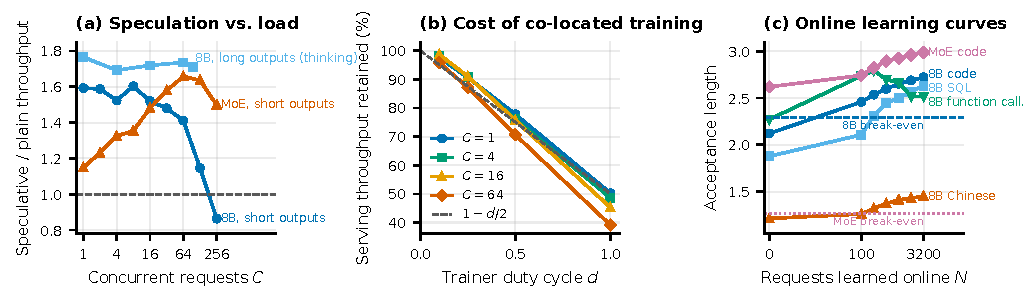
\includegraphics[width=\linewidth]{figures/fig1_motivation.pdf}
\caption{Calibration measurements (one H100, vLLM 0.27.1, factory EAGLE-3 drafters, $k{=}3$). (a) Speculative over plain-decoding throughput versus concurrency. (b) Serving throughput retained when a trainer shares the GPU at duty cycle $d$ (Qwen3-8B, short outputs, speculation on); the dashed line is $1-d/2$. (c) Acceptance length after learning online from $N$ requests; dashed lines mark the break-even acceptance at $C{=}256$ (Qwen3-8B code: \nv{astar.code.c256}; MoE code: \nv{astar.moe.c256}).}
\label{fig:motivation}
\end{figure*}

\section{Background and Measurements}\label{sec:measure}

\paragraph{Speculation and its break-even point.} A drafter proposes $k$ tokens and the target verifies them in one step, keeping the longest accepted prefix plus one token of its own. We use EAGLE-3 drafters \citep{li2025eagle3} with $k{=}3$, so the acceptance length $a$, the number of tokens emitted per verification step, lies between 1 and 4. At concurrency $C$ (requests being decoded), speculation is profitable when its throughput exceeds that of plain decoding, i.e., when the ratio $G(a,C)$ of the two exceeds one. Verification makes every step more expensive, and at high concurrency the GPU has no spare compute to absorb this cost, so the break-even acceptance $a^{*}(C)$ at which $G=1$ rises with load.

\paragraph{Measurement setup.} The measurements in this section use vLLM 0.27.1 on one H100 GPU, greedy decoding, the factory EAGLE-3 drafters for Qwen3-8B and Qwen3-30B-A3B released with AngelSlim \citep{yang2025qwen3,angelslim}, five short-output domains (chat, SQL, code, Chinese, function calling) and MATH-500 with thinking for long outputs (\cref{app:workloads}). They are the calibration inputs of the controller and were taken before the evaluation checkpoint was frozen (\cref{sec:setup}).

\paragraph{Whether speculation pays depends on load and architecture.} Figure~\ref{fig:motivation}a sweeps concurrency. For Qwen3-8B with short outputs, speculation is \nv{sweep.short.c1}\% faster than plain decoding at $C{=}1$ but \nv{sweep.short.c256abs}\% slower at $C{=}256$; with long outputs it remains \nv{sweep.long.c96}\% faster at the largest load we could run ($C{=}96$). The MoE target behaves the other way: the gain grows from \nv{sweep.moe.c1}\% at $C{=}1$ to \nv{sweep.moe.c64}\% at $C{=}64$ and is still \nv{sweep.moe.c256}\% at $C{=}256$. At $C{=}256$ a speculative step costs \nv{step.m2.c256}$\times$ a plain step on the MoE target but \nv{step.m1.c256}$\times$ on the dense one, consistent with the observation that sparse MoE targets profit from speculation at larger batches \citep{huang2025moesd}. A rule such as ``disable speculation under heavy load'' is right for one target and badly wrong for the other.

\paragraph{Co-located training is not free.} The trainer shares the GPU by time slicing: at duty cycle $d$ it computes for a fraction $d$ of the time. Serving throughput falls almost linearly, by $\kappa(C)\,d$ with $\kappa$ between \nv{kappa.min} and \nv{kappa.max} (Figure~\ref{fig:motivation}b): duty 0.1 costs \nv{duty.d01.lossmin}--\nv{duty.d01.lossmax}\% of throughput, duty 0.5 costs \nv{duty.d05.lossmin}--\nv{duty.d05.lossmax}\%, and training all the time costs \nv{duty.d10.lossmin}--\nv{duty.d10.lossmax}\% and raises p99 time per output token (TPOT) by \nv{duty.d10.p99min}--\nv{duty.d10.p99max}\%.

\paragraph{Learning ceilings differ.} Figure~\ref{fig:motivation}c shows the acceptance length after learning online from $N$ requests, one pass in arrival order, with the target's outputs as labels. Code and SQL improve steadily. Chinese stalls at \nv{lc.zh.n3200}, because only \nv{cover.zh}\% of the target's output tokens are in the drafter's 32k vocabulary. Function calling peaks at $N{=}\nv{lc.fc.peakN}$ and then declines. Against the break-even line at $C{=}256$, the code drafter crosses after about 100 requests, the Chinese drafter never does, and the MoE drafter is above its much lower break-even (\nv{astar.moe.c256}) from the start.

\paragraph{The profitability frontier.} For each domain $\ell$ we measured the throughput ratio of three or four drafter checkpoints at six loads. At every load the ratio is close to linear in acceptance (\cref{app:calibration}, Figure~\ref{fig:frontier}), so we fit
\begin{equation}
\Ghat_\ell(a,C)=\alpha_\ell(C)\,a+\beta_\ell(C),\qquad a^{*}_\ell(C)=\frac{1-\beta_\ell(C)}{\alpha_\ell(C)},\label{eq:frontier}
\end{equation}
with residuals of at most \nv{astar.code.err} for code, \nv{astar.zh.err} for Chinese, and \nv{astar.moe.err} for MoE code (\nv{astar.sql.err} at one SQL load). For Qwen3-8B the break-even acceptance rises from 1.0--1.2 at low load to \nv{astar.code.c256} (code), \nv{astar.sql.c256} (SQL), and \nv{astar.zh.c256} (Chinese) at $C{=}256$; for the MoE target it is \nv{astar.moe.c256}. The adapted code drafter reaches \nv{fr.code.n3200.c256}$\times$ plain decoding at $C{=}256$ in this sweep, whereas the factory drafter reaches \nv{fr.code.n0.c256}$\times$.

\section{Controller}\label{sec:method}

\paragraph{Setting.} One GPU serves a target model with an EAGLE-3 drafter and also runs a trainer that updates a copy of the drafter from features exported during serving (\cref{sec:system}). Every second the controller reads the number of running requests $C$, whether requests are queued, the acceptance length (smoothed by an exponential moving average, $\hat a$), the mean TPOT over the last second, and the trainer's progress. An operator-provided label $\ell$ names the current traffic domain, for example a product line; a \emph{regime} is a period with one label. The controller sets whether speculation is enabled ($z\in\{0,1\}$), the trainer's duty cycle $d\in\mathcal D=\{0,0.1,0.25,0.5,1\}$, and when the trainer exports a drafter, which is then hot-swapped into the server. The SLO bounds TPOT by twice the single-request decode time, $\Tslo$ (\nv{slo.m1}\,ms for Qwen3-8B, \nv{slo.m2}\,ms for the MoE target). Figure~\ref{fig:controller} summarizes the loop.

\paragraph{Calibration.} Before deployment we measure, once per target, the plain and speculative step times and plain throughput as functions of $C$, the interference coefficient $\kappa(C)$ (serving throughput falls by $\kappa(C)\,d$ at duty $d$), and the trainer's token rate $r$ at full duty; and once per domain, the frontier $\Ghat_\ell$ of \cref{eq:frontier} and the learning curve $a_\ell(N)$, the acceptance after learning from $N$ requests (\cref{sec:measure}). From these the controller predicts the throughput $\Theta(a,z,C)$ and the TPOT for any acceptance, speculation state, and duty. It never trains on a domain without a learning curve.

\paragraph{When to speculate.} Speculation is enabled when the current drafter beats plain decoding at the current load,
\begin{equation}
z=\mathbf{1}\big[\Ghat_\ell(\hat a,C)>1\big]\wedge\big(\widehat T_{\mathrm{spec}}\le\Tslo\vee\widehat T_{\mathrm{plain}}>\Tslo\big),\label{eq:switch}
\end{equation}
where the second clause keeps plain decoding if speculation would push an otherwise compliant load out of the SLO. A switch takes effect after three consecutive one-second ticks agree, and at most once every 10\,s. Acceptance cannot be measured while speculation is off, so after every drafter swap the controller turns speculation on for 8\,s to measure the new drafter.

\paragraph{Whether training can pay at all.} Let $\amax_\ell=\max_N a_\ell(N)$ be the domain's ceiling. If even the ceiling loses to plain decoding at the current load, $\Ghat_\ell(\amax_\ell,C)\le1$, no amount of training makes speculation worthwhile: the controller does not train, and \cref{eq:switch} turns speculation off instead (the \emph{structural-ceiling} test). Training also stops when the drafter is within 0.02 of its ceiling, or when the last swapped drafter raised the measured acceptance by less than 0.02.

\paragraph{How much to train.} If TPOT is within the SLO and no request is queued, the GPU has spare capacity and training costs latency but no throughput. The controller then picks the largest $d\in\mathcal D$ whose predicted TPOT stays below $0.9\,\Tslo$, i.e., $T_0/(1-\kappa(C)\,d)\le0.9\,\Tslo$, where $T_0$ is the measured TPOT with the slowdown of the current duty removed. Under saturation (requests queued, or $C$ at 95\% of the batch limit), training costs throughput immediately. The controller sets a target acceptance $a^{\dagger}=\hat a+0.8\,(\amax_\ell-\hat a)$, reads from the learning curve how many training tokens $n$ separate $\hat a$ from $a^{\dagger}$, and scores each $d\le0.5$ by
\begin{equation}
\begin{aligned}
V(d)={}&\big[\Theta^{\star}(a^{\dagger})-\Theta(\hat a)\big]\,\max\!\big(0,\widehat H-\tau(d)\big)\\
&-\Theta(\hat a)\,\kappa(C)\,b(d)\,\tau(d).
\end{aligned}\label{eq:value}
\end{equation}
Here $\tau(d)=n/\min(rd,\rho)$ is the training time when training data become available at rate $\rho$, $b(d)=\min(d,\rho/r)$ is the trainer's actual busy fraction, $\Theta^{\star}$ is the better of speculation on and off, and $\widehat H$ is the forecast remaining length of the regime. The first term is the throughput gained once the improved drafter is in place; the second is the throughput lost while it trains. The controller trains at $\arg\max_d V(d)$ if the maximum is positive and not at all otherwise. Because it does not know when the regime will end, it forecasts $\widehat H$ as the time the regime has lasted so far, clipped to $[90,600]$\,s.

\paragraph{Export and swap.} The trainer exports a drafter after 100, 200, 400, \dots{} requests learned in the current regime, and each export is swapped in immediately. When the label changes, the trainer's buffer is flushed and the schedule restarts.

\paragraph{What the controller assumes.} It needs the domain label and a per-domain calibration, which a short profiling run provides. It does not know when the regime will end or when training should stop. The rules and their constants (\cref{app:controller}) were fixed during development runs before the evaluation checkpoint was frozen and were not changed afterwards.

\begin{figure*}[t]
\centering
% Control loop of the controller (Section 3). TikZ; needs positioning, arrows.meta, calc, fit.
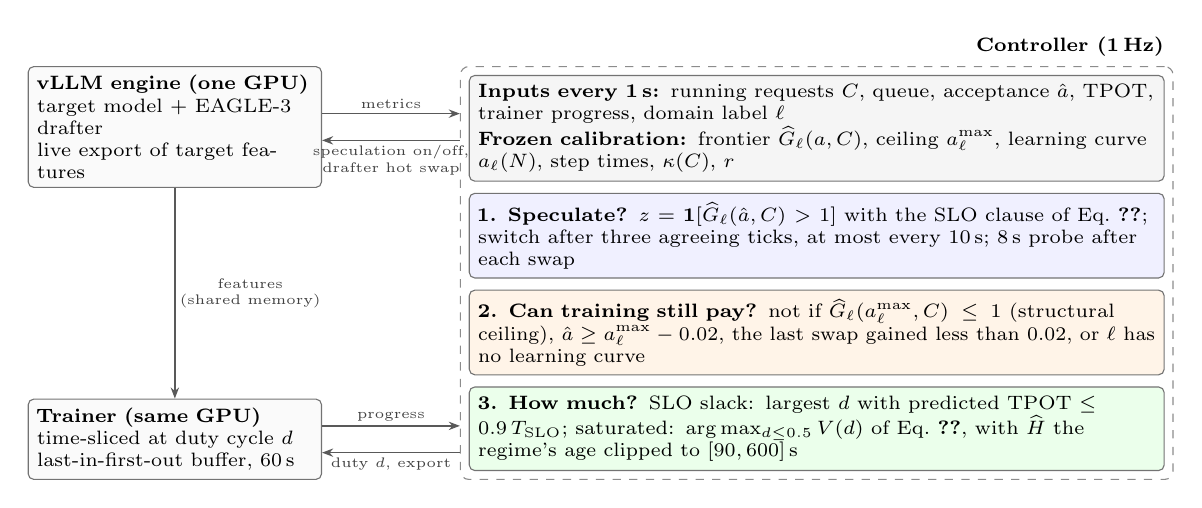
\begin{tikzpicture}[
  font=\scriptsize, >={Stealth[length=4pt]}, node distance=4pt,
  box/.style={draw=black!55, rounded corners=2pt, align=left, inner sep=3.2pt, text width=#1},
  arr/.style={->, draw=black!65, line width=0.6pt},
  lab/.style={font=\tiny, text=black!75, align=center, inner sep=1.5pt},
]
% controller (right)
\node[box=8.6cm, fill=black!4] (in) {%
  {\bfseries Inputs every 1\,s:} running requests $C$, queue, acceptance $\hat a$, TPOT, trainer progress, domain label $\ell$\\
  {\bfseries Frozen calibration:} frontier $\Ghat_\ell(a,C)$, ceiling $\amax_\ell$, learning curve $a_\ell(N)$, step times, $\kappa(C)$, $r$};
\node[box=8.6cm, fill=blue!6, below=of in] (r1) {%
  {\bfseries 1. Speculate?}\enspace $z=\mathbf{1}[\Ghat_\ell(\hat a,C)>1]$ with the SLO clause of Eq.~\ref{eq:switch}; switch after three agreeing ticks, at most every 10\,s; 8\,s probe after each swap};
\node[box=8.6cm, fill=orange!9, below=of r1] (r2) {%
  {\bfseries 2. Can training still pay?}\enspace not if $\Ghat_\ell(\amax_\ell,C)\le1$ (structural ceiling), $\hat a\ge\amax_\ell-0.02$, the last swap gained less than 0.02, or $\ell$ has no learning curve};
\node[box=8.6cm, fill=green!8, below=of r2] (r3) {%
  {\bfseries 3. How much?}\enspace SLO slack: largest $d$ with predicted TPOT $\le0.9\,\Tslo$; saturated: $\arg\max_{d\le0.5}V(d)$ of Eq.~\ref{eq:value}, with $\widehat H$ the regime's age clipped to $[90,600]$\,s};
\node[draw=black!45, dashed, rounded corners=3pt, fit=(in)(r3), inner sep=3pt] (ctl) {};
\node[font=\scriptsize\bfseries, anchor=south east] at (ctl.north east) {Controller (1\,Hz)};
% serving engine and trainer (left)
\node[box=3.5cm, fill=black!2, anchor=north east] (eng) at ($(ctl.north west)+(-1.75cm,0)$) {%
  {\bfseries vLLM engine (one GPU)}\\ target model + EAGLE-3 drafter\\ live export of target features};
\node[box=3.5cm, fill=black!2, anchor=south east] (trn) at ($(ctl.south west)+(-1.75cm,0)$) {%
  {\bfseries Trainer (same GPU)}\\ time-sliced at duty cycle $d$\\ last-in-first-out buffer, 60\,s};
\draw[arr] (eng.south) -- node[lab, right]{features\\(shared memory)} (trn.north);
% plant <-> controller
\draw[arr] ($(eng.east)+(0,0.17)$) -- node[lab, above]{metrics} ($(ctl.west |- eng.east)+(0,0.17)$);
\draw[arr] ($(ctl.west |- eng.east)+(0,-0.17)$) -- node[lab, below]{speculation on/off,\\drafter hot swap} ($(eng.east)+(0,-0.17)$);
\draw[arr] ($(trn.east)+(0,0.17)$) -- node[lab, above]{progress} ($(ctl.west |- trn.east)+(0,0.17)$);
\draw[arr] ($(ctl.west |- trn.east)+(0,-0.17)$) -- node[lab, below]{duty $d$, export} ($(trn.east)+(0,-0.17)$);
\end{tikzpicture}

\caption{The control loop. Each second the controller combines engine and trainer measurements with the frozen calibration and applies three tests: whether the current drafter beats plain decoding (\cref{eq:switch}), whether training can still pay (structural ceiling, ceiling, convergence), and how much to train (SLO slack, or the value of \cref{eq:value} under saturation). Its outputs are a speculation switch, the trainer's duty cycle, and drafter exports that are hot-swapped into the running engine.}
\label{fig:controller}
\end{figure*}

\section{Implementation}\label{sec:system}

We implement the system on vLLM 0.27.1 (V1 engine) with three engine extensions and two processes beside the server.

\paragraph{Live feature export.} The trainer needs the target's auxiliary hidden states at every accepted position. Inside the EAGLE-3 path of the model runner, we copy them from the GPU to pinned host memory without blocking the step, and a background thread writes them per request into a shared-memory ring buffer. Rejected draft positions are dropped, only tensor-parallel rank 0 writes, and when the buffer is full the exporter drops one step and marks the gap instead of stalling serving. Prefix caching has to be disabled, because positions served from the cache have no hidden states.

\paragraph{Trainer.} A separate process on the same GPU trains the drafter with cross-entropy against the target's own next tokens over the drafter's vocabulary (AdamW, learning rate $5\times10^{-5}$, about 4{,}096 tokens per step). It reads completed requests from the ring buffer into a last-in-first-out buffer of at most 600k tokens, discards data older than 60\,s, and implements duty cycle $d$ by sleeping $(1-d)/d$ times the duration of each step. Data are not the bottleneck: the trainer consumed only \nv{zh.full.usedpct}--\nv{moe.full.usedpct}\% of the requests served in a run (\cref{app:extra}).

\paragraph{Drafter hot swap and speculation switch.} A collective RPC loads new drafter weights into all workers without restarting the engine; in the frozen runs a swap took a median of \nv{swap.m1.med}\,s for the Qwen3-8B drafter and \nv{swap.m2.med}\,s for the MoE drafter. A second RPC switches speculation in the scheduler and the workers together, so drafting stops instead of being computed and discarded; the drafter stays in GPU memory and the round trip takes a median of \nv{switch.med}\,ms.

\paragraph{Controller.} The controller is a 1\,Hz process that reads the engine's metrics endpoint and the trainer's log, writes the duty cycle to a file that the trainer reads before every step, and requests exports through a command file.

\section{Evaluation}\label{sec:evaluation}

\subsection{Setup}\label{sec:setup}

\paragraph{One frozen checkpoint.} Every experiment in this section runs on one checkpoint that we froze before the first run: the controller, trainer, and harness code, the six patched engine files, the two calibration files, the factory drafters, the target weights, the prompt pools, the seeds, and the software environment, each recorded by hash (\cref{app:manifest}). The simulator of \cref{sec:heldout} reads the same frozen calibration file.

\paragraph{Workload.} Each run serves three phases on one H100 GPU: 200 chat requests at concurrency 16 (phase A1), then 16{,}000 unique requests from a new domain at concurrency 256, which saturate the GPU for \nv{bdur.min}--\nv{bdur.max}\,s (phase B), then 200 different chat requests (phase A2). The three scenarios are Qwen3-8B with code in B, Qwen3-8B with Chinese in B, and Qwen3-30B-A3B with code in B. Decoding is greedy, outputs stop naturally or at 512 tokens, and the B prompts were never seen during calibration. Every policy except the production reference reserves the trainer's memory (18\,GB for Qwen3-8B and 5\,GB for the MoE target), and every such policy that loads a drafter also runs the export path.

\paragraph{Policies.} \pol{Production} runs the factory drafter with speculation always on, without export or memory reserve, as deployed today. \pol{Static} does the same under the evaluation's engine configuration and is the reference for all differences. \pol{Plain} serves without a drafter. \pol{Switch} applies \cref{eq:switch} with the domain's frontier and never trains. \pol{Threshold} turns speculation off whenever the server is saturated and trains at duty 0.5 whenever TPOT is within the SLO, i.e., the idle-time rule of OSD \citep{liu2024osd} combined with a load threshold. \pol{Always} trains at duty 0.5 from the first request and swaps drafters after 100, 200, 400, \dots{} requests. \pol{Informed} trains at duty 0.5 from the moment phase B starts until it has learned from 800 requests, swapping at 100, 200, 400, and 800; we chose its stopping point from the learning curves of \cref{fig:motivation}c, so it is a reference that knows when to stop rather than a deployable policy. \pol{Full} is the controller of \cref{sec:method}. \pol{Always} and \pol{Informed} never turn speculation off (\cref{app:policies}).

\paragraph{Repetitions and metrics.} Every policy runs three times per scenario. Repetition $r$ fixes the prompt order of all phases and the trainer's random seed, so within a repetition all policies serve the same request sequence, and we report paired differences as mean $\pm$ standard deviation over the three pairs. The main metric is output throughput during phase B; we also report TPOT and the throughput of the whole run. The \nv{n.runs} runs used \nv{gpuh} GPU-hours on \nv{hosts} nodes of the same type; the coefficient of variation of B throughput was at most \nv{cv.static.max}\% for the static policies.

\subsection{The best policy differs by scenario}\label{sec:results}

\begin{table*}[t]
\caption{Phase-B (saturated) throughput relative to \pol{Static}: paired mean $\pm$ standard deviation over three repetitions, in percent. Parentheses give mean throughput as a fraction of the best policy in that scenario (bold); the \pol{Static} row gives absolute throughput. The last column is the smallest fraction over the three scenarios.}
\label{tab:main}
\centering\small
% generated by code/specsched/paper_assets.py -- do not edit by hand
\begin{tabular}{@{}lcccc@{}}
\toprule
Policy & 8B code & 8B Chinese & MoE code & Worst case\\
\midrule
Production speculation & $+2.2$\,$\pm$0.9 \,{\scriptsize(0.854)} & $+1.8$\,$\pm$0.8 \,{\scriptsize(0.517)} & $+1.0$\,$\pm$0.1 \,{\scriptsize(0.923)} & 0.517 \\
Static speculation & 14{,}282 tok/s \,{\scriptsize(0.835)} & 8{,}526 tok/s \,{\scriptsize(0.508)} & 13{,}859 tok/s \,{\scriptsize(0.915)} & 0.508 \\
Plain decoding & $+18.1$\,$\pm$0.9 \,{\scriptsize(0.986)} & \textbf{\boldmath $+97.0$\,$\pm$1.4 \,{\scriptsize(1.000)}} & $-46.1$\,$\pm$0.1 \,{\scriptsize(0.493)} & 0.493 \\
\addlinespace[2pt]
Switch only & $+12.9$\,$\pm$2.5 \,{\scriptsize(0.943)} & $+90.9$\,$\pm$2.2 \,{\scriptsize(0.969)} & $-0.3$\,$\pm$0.3 \,{\scriptsize(0.912)} & 0.912 \\
Threshold rule & $+14.8$\,$\pm$0.8 \,{\scriptsize(0.959)} & $+86.9$\,$\pm$4.7 \,{\scriptsize(0.949)} & $-46.0$\,$\pm$0.0 \,{\scriptsize(0.494)} & 0.494 \\
TIDE-style triggers & $+13.8$\,$\pm$3.5 \,{\scriptsize(0.950)} & $+54.5$\,$\pm$3.6 \,{\scriptsize(0.784)} & $+6.0$\,$\pm$4.0 \,{\scriptsize(0.970)} & 0.784 \\
\addlinespace[2pt]
Always train & $+2.4$\,$\pm$1.9 \,{\scriptsize(0.855)} & $-1.2$\,$\pm$0.7 \,{\scriptsize(0.502)} & $-3.6$\,$\pm$0.3 \,{\scriptsize(0.882)} & 0.502 \\
Informed schedule & \textbf{\boldmath $+19.7$\,$\pm$0.5 \,{\scriptsize(1.000)}} & $+13.8$\,$\pm$0.4 \,{\scriptsize(0.578)} & \textbf{\boldmath $+9.3$\,$\pm$0.7 \,{\scriptsize(1.000)}} & 0.578 \\
\rowcolor{resultgraylight}Full controller & $+18.0$\,$\pm$1.6 \,{\scriptsize(0.985)} & $+87.7$\,$\pm$8.5 \,{\scriptsize(0.953)} & $+8.0$\,$\pm$0.4 \,{\scriptsize(0.988)} & \textbf{0.953} \\
\bottomrule
\end{tabular}

\end{table*}

\begin{figure*}[t]
\centering
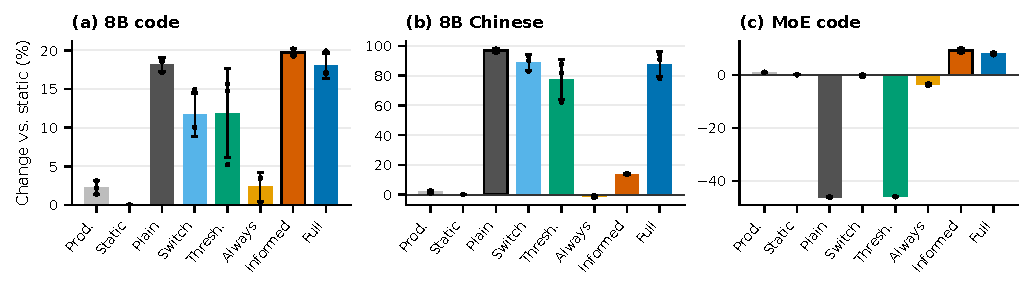
\includegraphics[width=\linewidth]{figures/fig4_policies.pdf}
\caption{Phase-B throughput change relative to \pol{Static} per repetition (dots), with the paired mean and standard deviation (bars). The best policy in each scenario has a black outline. Prod.: \pol{Production}; Thresh.: \pol{Threshold}.}
\label{fig:policies}
\end{figure*}

Table~\ref{tab:main} and Figure~\ref{fig:policies} show the frozen matrix. The best policy is \pol{Plain} for Qwen3-8B Chinese and \pol{Informed} for both code scenarios, and every policy other than \pol{Full} falls well short in at least one scenario. \pol{Plain} and \pol{Threshold} lose about half of the MoE throughput, because they turn speculation off where it is still \nv{fr.moe.n0.c256}$\times$ faster than plain decoding. \pol{Informed} keeps speculating on Chinese and reaches only \nv{zh.informed.r} of \pol{Plain}. \pol{Switch}, which never trains, is the most robust alternative but still falls \nv{switch.worstshort}\% short on MoE. \pol{Full} is the only policy within 5\% of the best in every scenario (worst case \nv{full.worst}). Against \pol{Static} it raises phase-B throughput by \nv{code.full.d}$\pm$\nv{code.full.sd}\%, \nv{zh.full.d}$\pm$\nv{zh.full.sd}\%, and \nv{moe.full.d}$\pm$\nv{moe.full.sd}\%, with the same sign in every repetition, and over the whole run it is \nv{code.full.session}\%, \nv{zh.full.session}\%, and \nv{moe.full.session}\% faster than \pol{Production}.

\subsection{Which lever the controller pulls}\label{sec:levers}

\begin{table*}[t]
\caption{What \pol{Full} did during phase B (means over three runs): fraction of time with speculation on, mean duty cycle, drafter swaps, acceptance length at the start and end of B, tokens trained over the whole run, and the decisions of the training tests, as a share of one-second ticks (shares below 5\% omitted).}
\label{tab:behaviour}
\centering\small
% generated by code/specsched/paper_assets.py -- do not edit by hand
\begin{tabularx}{\linewidth}{@{}lccccc>{\raggedright\arraybackslash}X@{}}
\toprule
Scenario & Spec.\ on & Duty & Swaps & Acceptance & Train tok.\ (M) & Decisions during the saturated phase (share of 1\,s ticks)\\
\midrule
8B code & 100\% & 0.067 & 3 & 2.50$\to$2.66 & 0.64 & no training (value $\le 0$) 77\%, train (value $>0$) 10\%, converged 10\% \\
8B Chinese & 2\% & 0.016 & 1 & 1.18$\to$1.18 & 0.38 & structural ceiling 97\% \\
MoE code & 100\% & 0.084 & 4 & 2.68$\to$2.97 & 0.81 & at ceiling 43\%, no training (value $\le 0$) 36\%, train (value $>0$) 19\% \\
\bottomrule
\end{tabularx}

\end{table*}

Table~\ref{tab:behaviour} shows that the controller takes qualitatively different actions in the three scenarios.

\paragraph{Chinese: turn speculation off.} The structural-ceiling test decides \nv{zh.full.why.structural_ceiling}\% of the ticks: even the best reachable drafter (\nv{lc.zh.n3200}) is below break-even at this load, so the controller keeps speculation off except for short probes and spends almost no time training (mean duty \nv{zh.full.duty}). Relative to \pol{Plain} it ends at \nv{zh.full_vs_plain}\%: the engine's speculation-off state is slower than serving without a drafter (\pol{Switch} ends at \nv{zh.switch_vs_plain}\%), and the first seconds of B are served with speculation on. \pol{Informed}, which cannot turn speculation off, spends its training on a drafter that can never pay; \pol{Full} is \nv{zh.full_vs_informed}\% relative to it.

\paragraph{Qwen3-8B code: adapt and keep speculating.} The controller never turns speculation off. It enters phase B with acceptance \nv{code.full.acc0} instead of the factory \nv{code.static.acc0}, because it already trained in the SLO slack of phase A1 and the chat-trained drafter transfers to code; during B it trains at a mean duty of \nv{code.full.duty}, swaps \nv{code.full.swaps} drafters, and reaches \nv{code.full.acc1}. The value rule of \cref{eq:value} declines to train in \nv{code.full.why.saturated_no_value}\% of the phase-B ticks. The adapted drafter makes speculation as fast as plain decoding at $C{=}256$ (\nv{code.full_vs_plain}\%). This is \nv{code.full_vs_switch}$\pm$\nv{code.full_vs_switch.sd}\% relative to \pol{Switch}, about as much as the engine's speculation-off state costs (\pol{Switch} is \nv{code.switch_vs_plain}\% relative to \pol{Plain}); \pol{Plain}, which has no such overhead, is as fast as \pol{Full} here. For a dense target at saturation, adaptation thus mainly lets speculation escape the regime where the factory drafter loses.

\paragraph{MoE code: adaptation is the whole gain.} Turning speculation off would halve throughput, and the controller keeps it on. It trains at a mean duty of \nv{moe.full.duty}, swaps \nv{moe.full.swaps} drafters, raises acceptance from \nv{moe.full.acc0} to \nv{moe.full.acc1}, and then stops at the ceiling (\nv{moe.full.why.at_ceiling}\% of ticks). Its \nv{moe.full.d}\% over \pol{Static} comes entirely from adaptation: relative to \pol{Switch} it is \nv{moe.full_vs_switch}$\pm$\nv{moe.full_vs_switch.sd}\%, while \pol{Threshold}, whose load rule turns speculation off, loses \nv{moe.thresh.abs}\%.

\paragraph{Against the informed schedule.} Where adaptation pays, \pol{Informed} is slightly faster. Relative to it, \pol{Full} is \nv{code.full_vs_informed}\% on Qwen3-8B code, within the run-to-run spread (\nv{code.full_vs_informed.min} to \nv{code.full_vs_informed.max}\% per repetition), and \nv{moe.full_vs_informed}\% on MoE, with the same sign in all three repetitions (\nv{moe.full_vs_informed.min} to \nv{moe.full_vs_informed.max}\%). It trains at duty 0.5 from the first second of B, whereas the controller raises its duty only when \cref{eq:value} is positive. \pol{Always}, which never stops training, ends close to \pol{Static} (\nv{code.always.d}\%, \nv{zh.always.d}\%, \nv{moe.always.d}\%): continuous training costs as much throughput as the better drafter gains. We therefore do not claim that the controller beats a well-chosen fixed schedule where one exists; it matches such schedules within 1.5\% without knowing when to stop, and it does not fail where they do.

\subsection{Latency}\label{sec:latency}

Faster serving under saturation also shortens tail latency: relative to \pol{Static}, \pol{Full} changes phase-B p99 TPOT by \nv{code.full.p99}\%, \nv{zh.full.p99}\%, and \nv{moe.full.p99}\% (\cref{tab:latency} in \cref{app:extra}). The light phases show the price of training in the SLO slack. On Qwen3-8B, the median TPOT of phase A1 changes by \nv{code.full.a1}\% and \nv{zh.full.a1}\%, still far below the \nv{slo.m1}\,ms SLO, and in phase A2 \pol{Full} stays close to \pol{Static} (\nv{code.full.a2}\%, \nv{zh.full.a2}\%) because it keeps training in the slack; \pol{Informed}, which has stopped training and kept its adapted drafter, changes A2 TPOT by \nv{code.informed.a2}\% and \nv{zh.informed.a2}\%. On the MoE target the calibration contains no chat learning curve, so \pol{Full} never trains in the chat phases, and its code-adapted drafter changes A2 TPOT by \nv{moe.full.a2}\% (\pol{Informed}: \nv{moe.informed.a2}\%). Spending slack on training serves throughput; a latency-oriented deployment would cap the duty in the slack rule.

\subsection{Held-out validation in a frozen simulator}\label{sec:heldout}

\begin{figure*}[t]
\centering
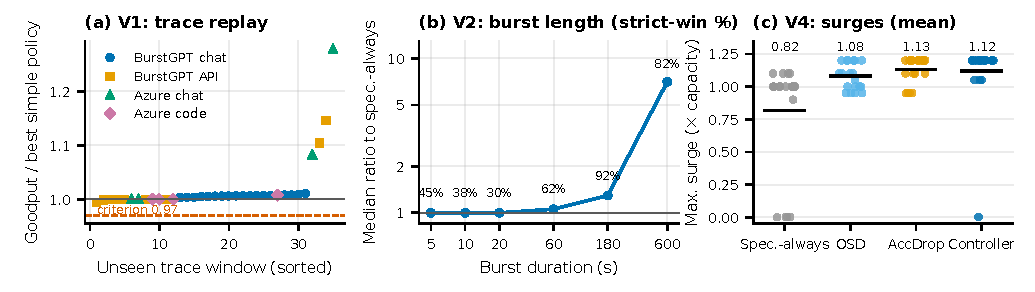
\includegraphics[width=\linewidth]{figures/fig5_heldout.pdf}
\caption{Frozen-simulator validation on unseen workloads. (a) Goodput of the controller relative to the best of five simple policies in each of \nv{v1.n} trace windows (sorted). (b) Median goodput relative to \pol{SpecAlways} for bursts of a new domain, by burst length; labels give the share of strict wins. (c) Largest surge, in multiples of plain-decoding capacity, served without SLO violation in 20 scenarios (dots) and their mean (bars).}
\label{fig:heldout}
\end{figure*}

The live runs cover one workload shape. To test other traffic, we replay traces in a simulator built from the same frozen calibration file: a fluid single-GPU model in which arrivals set the operating concurrency, excess demand queues, training slows serving by $\kappa(C)\,d$, and acceptance follows the measured learning curves, including the measured transfer to chat. The simulator implements the controller's rules, with goodput (tokens served within the SLO) instead of throughput as the currency under saturation, and five simple policies: \pol{NoSpec}, \pol{SpecAlways}, and three that keep speculation on and train at full duty when a trigger fires: \pol{OSD} (fewer than 16 running requests), \pol{Timed} (30\,s every 5 minutes), and \pol{AccDrop} (acceptance below 95\% of the ceiling, an acceptance-triggered rule in the spirit of TIDE). We froze the simulator and the calibration (hashes \texttt{\nv{sim.hash}} and \texttt{\nv{model.hash}}) and declared four criteria before running workloads never used in development: \nv{v1.n} trace windows from BurstGPT \citep{wang2024burstgpt} chat and API logs on days we had not replayed and from the Azure 2023 chat and code traces \citep{patel2024splitwise}, each at three or four load scales; 60 random bursts of a new domain; 40 Chinese regimes; and 20 surge scenarios at seven surge levels (\cref{app:sim}).

Figure~\ref{fig:heldout} and \cref{tab:heldout} in \cref{app:sim} report the outcomes. The goodput criterion holds in all \nv{v1.n} trace windows: the controller is never more than \nv{v1.short}\% below the best simple policy and is the best policy in \nv{v1.best}. It trains on \nv{v1.cmtrain.min}--\nv{v1.cmtrain.max}M tokens per trace window, whereas \pol{OSD} trains on up to \nv{v1.osdtrain.max}M; the training criterion fails only in four Azure chat windows, where \pol{OSD} itself trains on fewer tokens than the controller. Three expectations did not survive. First, training pays back reliably only for long bursts: short bursts are mostly ties, strict wins reach \nv{v2.d60.win}\% at 60\,s and \nv{v2.d180.win}\% at 180\,s. Second, the controller ranks above \pol{SpecAlways}, \pol{OSD}, and \pol{AccDrop} in all \nv{v3.n} Chinese regimes, but its advantage over \pol{SpecAlways} is \nv{v3.feas.min}--\nv{v3.feas.max}$\times$ at feasible saturation and as low as \nv{v3.over.min}$\times$ under overload, so the pre-declared $1.5\times$ margin fails. Third, \pol{AccDrop} tolerates surges as well as the controller (mean \nv{v4.acc} versus \nv{v4.cm}); the controller's advantage lies in meeting all four criteria at once. Finally, the horizon forecast barely matters in these workloads: replacing it with the true remaining length of the regime changes the outcome in \nv{hz.diff} of \nv{hz.total} cases.

\subsection{Overheads}\label{sec:overheads}

The export path and the trainer's memory reserve cost \nv{moe.infra}--\nv{code.infra}\% of phase-B throughput (\pol{Production} versus \pol{Static}). The engine's speculation-off state is \nv{zh.switch_vs_plain.abs}--\nv{code.switch_vs_plain.abs}\% slower than serving without a drafter. Part of the gap is the first seconds of phase B, which are served with speculation on; the rest is the cost of keeping the drafter loaded while speculation is off, which we did not separate further. It is the largest overhead and a target for engine work. Drafter swaps (\nv{swap.m1.min}--\nv{swap.m1.max}\,s for Qwen3-8B, \nv{swap.m2.min}--\nv{swap.m2.max}\,s for MoE) and speculation switches (at most \nv{switch.max}\,ms) did not cause a single failed request in the \nv{n.runs} runs (\cref{app:extra}).

\section{Related Work}\label{sec:related}

\paragraph{Speculative decoding and drafters.} Speculative decoding \citep{leviathan2023fast,chen2023accelerating} and tree-based verification \citep{miao2024specinfer} preserve the target's output distribution while emitting several tokens per step. Drafter designs range from extra decoding heads \citep{cai2024medusa} to feature-level drafters such as EAGLE, EAGLE-2, and EAGLE-3 \citep{li2024eagle,li2024eagle2,li2025eagle3}. MoESD \citep{huang2025moesd} and MagicDec \citep{sadhukhan2025magicdec} show that speculation keeps paying at larger batch sizes for sparse MoE targets and for long sequences, respectively, in line with our measurements.

\paragraph{Load-aware speculation control.} TurboSpec \citep{liu2024turbospec} chooses the speculation length, including zero, to maximize estimated goodput; AdaSpec \citep{huang2025adaspec} adapts speculation to latency SLOs; Nightjar \citep{li2025nightjar} uses a bandit planner to disable speculation when it stops paying and offloads the drafter; FASER \citep{chen2026faser} sets the speculation length of each request in a batch and overlaps drafting with verification. These systems control a fixed drafter; our frontier moves as the drafter trains and decides whether training pays.

\paragraph{Online drafter adaptation.} OSD \citep{liu2024osd} distills the drafter from the target's outputs when the server has spare capacity. OnlineSPEC \citep{qian2026drafts} casts drafter adaptation as online learning with dynamic-regret guarantees. Aurora \citep{wang2026aurora} trains the drafter from live traffic on a separate training server and hot-swaps it into the inference server. TIDE \citep{park2026tide} reuses the target's hidden states, trains on separate GPUs, enables speculation above a batch-dependent acceptance threshold, and triggers training when acceptance drifts. DVI \citep{bhansali2025dvi} trains a self-speculative drafter online from accept and reject signals. Others select among drafters online \citep{liu2026notabandit} or co-train the drafter with the policy during RL rollouts \citep{wang2026cotraining}. We differ in placing the trainer on the serving GPU, which turns every training decision into a trade against serving throughput, and in deciding how much to train and when to stop by the value of the resulting drafter, including whether it can ever cross break-even.

\section{Limitations}\label{sec:limitations}

\paragraph{Calibration and labels.} The controller needs an operator label for the traffic domain and a per-domain calibration of the frontier and the learning curve. On an unlabelled or uncalibrated domain it does not train; unlabelled production traffic needs online estimates of both, which we leave open.

\paragraph{Scope of the live evaluation.} We evaluate two engines, vLLM 0.27.1 and, with five of the \nv{n.pol} policies, SGLang 0.5.10, one GPU type (H100), two targets of one model family, EAGLE-3 drafters with $k{=}3$, greedy decoding with outputs of at most 512 tokens that end naturally (with every output forced to 256 tokens, the adapted code drafter reaches only \nv{proto.fixed.n3200}$\times$ plain decoding; \cref{tab:protocol}), single-GPU serving, and prefix caching disabled. Drafter hot swap was tested functionally with tensor parallelism before the freeze, but the controller was not evaluated there. \pol{TIDE} reimplements only TIDE's training triggers, on a shared GPU and with a live drafter comparison; TIDE itself trains on separate GPUs. The live workload is a synthetic chat--new-domain--chat sequence; other traffic shapes are covered only in simulation.

\paragraph{Statistics.} Each cell has three paired repetitions, and runs were spread over \nv{hosts} nodes of the same type. Node interference slowed \nv{scan.flagged.word} baseline runs, which we replaced by reruns (\cref{app:rerun}); smaller slowdowns remain in the data. Paired differences of a few percent between adaptive policies, such as \pol{Full} versus \pol{Informed} on Qwen3-8B code, are within the run-to-run spread.

\paragraph{Development and evaluation.} The rules and constants were developed on runs that drew from the same prompt pools as the frozen evaluation, in different orders. The frozen evaluation therefore does not test the constants on unseen prompts; the simulator validation on unseen traces only partly fills this gap, because it shares the calibration.

\section{Conclusion}\label{sec:conclusion}

A better drafter is worth training only if it will be used, and worth using only above break-even at the current load. Coupling a calibrated profitability frontier with learning curves picks the right lever in each scenario we tested: the controller turns speculation off when the drafter cannot reach break-even, adapts the drafter when speculation must stay on, and stops training when the expected gain no longer repays the capacity it costs. Dense and MoE targets need opposite actions at saturation: no other policy we tested stays within \nv{alt.minshort.floor}\% of the best in every scenario, while the controller stays within \nv{full.worstshort}\% without knowing when to stop.


\section*{Impact Statement}
This paper presents work whose goal is to make the serving of large language models more efficient. Serving the same traffic with fewer GPU-hours lowers the cost and energy use per request. We do not see consequences specific to this work beyond those of deploying language models in general.

\bibliography{refs}
\bibliographystyle{icml2026}

\newpage
\appendix
\onecolumn
\FloatBarrier
\section{Frozen Checkpoint and Configuration}\label{app:manifest}

All results of \cref{sec:evaluation} come from one checkpoint frozen before the first run. Table~\ref{tab:manifest} lists the hashes recorded in its manifest; the local copies of the controller, trainer, harness, calibration files, and simulator were checked against them when this paper's tables were generated. Every number in the paper is produced by one script from the run directories and the frozen files, not typed by hand.

\begin{table}[!htbp]
\caption{Hashes of the frozen checkpoint (first 16 hexadecimal digits of SHA-256).}
\label{tab:manifest}
\centering\small
% generated by code/specsched/paper_assets.py -- do not edit by hand
\begin{tabular}{@{}ll@{}}
\toprule
Component & SHA-256 (first 16 hex digits)\\
\midrule
\texttt{controller.py} & \texttt{0c526960ecb25143} \\
\texttt{train\_head.py} & \texttt{cc224db0c6b40c81} \\
\texttt{hotswap\_run.py} & \texttt{866e1159bda44604} \\
\texttt{livetap.py} & \texttt{719538857da7d833} \\
\texttt{sched/model.json} & \texttt{18c3723adbe9b858} \\
\texttt{sched/model\_m2.json} & \texttt{5c9fa2d452ca7156} \\
\texttt{sched/sim.py} & \texttt{451c5673bbb4c7a4} \\
\texttt{vllm/v1/worker/gpu\_model\_runner.py} (patched) & \texttt{08c3099b3f725380} \\
\texttt{vllm/v1/worker/gpu\_worker.py} (patched) & \texttt{ca3add781f3ab162} \\
\texttt{vllm/v1/core/sched/scheduler.py} (patched) & \texttt{a8670d8b381dde71} \\
\texttt{vllm/v1/engine/core.py} (patched) & \texttt{e9353a6d8cd9cfe4} \\
\texttt{vllm/v1/spec\_decode/live\_tap.py} (patched) & \texttt{cae550fdf2ad39d1} \\
\texttt{vllm/v1/worker/gpu/model\_runner.py} (patched) & \texttt{ade8b970f18d7533} \\
Drafter \texttt{qwen3-8b-eagle3} & \texttt{048b9c4ada5fc26a} \\
Drafter \texttt{qwen3-a3b-eagle3} & \texttt{dc6373b07e6eb6c1} \\
Target weights, Qwen3-8B / Qwen3-30B-A3B & \texttt{f7c4eadfbbf52247} / \texttt{2850ddb3bf7aecad} \\
Software & torch 2.13.0, transformers 5.15.1, triton 3.7.1, vllm 0.27.1 \\
\bottomrule
\end{tabular}

\end{table}

\paragraph{Engine.} vLLM 0.27.1 (V1 engine), one H100 GPU per run, \texttt{max\_num\_seqs} 256, maximum model length 4{,}096, prefix caching disabled, greedy decoding, outputs of at most 512 tokens with natural stopping. GPU memory utilization is \nv{util.prod} for \pol{Production} and 0.90 minus the trainer's reserve for all other policies (\nv{util.m1} for Qwen3-8B, \nv{util.m2} for the MoE target). EAGLE-3 drafters with $k{=}3$, auxiliary target layers $(2,18,33)$ for Qwen3-8B and $(2,24,45)$ for Qwen3-30B-A3B, and a 32k draft vocabulary. The feature export uses a 4\,GB shared-memory ring and samples every step.

\paragraph{Trainer.} Cross-entropy on the target's next tokens over the draft vocabulary; AdamW with learning rate $5\times10^{-5}$, betas $(0.9,0.95)$, no weight decay, 10 warm-up steps, and gradient clipping at 1.0; about 4{,}096 tokens per step and at most 2{,}048 tokens per sequence; a last-in-first-out buffer of at most 600k tokens with a 60\,s age limit; duty cycle by sleeping $(1-d)/d$ times the step time. The trainer's seed is the repetition index.

\FloatBarrier
\section{Workloads and Calibration}\label{app:calibration}

\subsection{Workloads}\label{app:workloads}

Table~\ref{tab:workloads} describes the domains. For calibration, each domain was deduplicated and shuffled, and the target generated greedy outputs for 3{,}200 training, 300 evaluation, and 300 reserve prompts. The prompts of phase B in the evaluation come from separate pools of unique prompts that exclude every calibration prompt (16{,}222 code and 44{,}776 Chinese prompts); phases A1 and A2 use two disjoint sets of 200 chat prompts per repetition.

\begin{table}[!htbp]
\caption{Domains. Token counts are means over the target's greedy outputs (Qwen3-8B); \emph{Truncated} is the share of outputs that hit the 512-token limit; \emph{Coverage} is the share of target output tokens inside the 32k draft vocabulary. MATH-500 is used only for the long-output sweep, with thinking enabled and outputs of up to 4{,}096 tokens.}
\label{tab:workloads}
\centering\footnotesize\setlength{\tabcolsep}{4pt}
% generated by code/specsched/paper_assets.py -- do not edit by hand
\begin{tabularx}{\linewidth}{@{}l>{\raggedright\arraybackslash}Xrrrrr@{}}
\toprule
Domain & Source & Prompts & Prompt tok. & Output tok. & Truncated & Coverage\\
\midrule
Chat & UltraChat 200k \citep{ding2023ultrachat} & 3{,}800 & 109 & 439 & 73.7\% & 95.8\% \\
SQL & sql-create-context \citep{sqlcreatecontext} & 3{,}800 & 68 & 27 & 0.0\% & 91.5\% \\
Code & CodeAlpaca-20k \citep{codealpaca} & 3{,}800 & 38 & 275 & 15.5\% & 97.6\% \\
Chinese & alpaca-gpt4-zh \citep{peng2023gpt4instruct} & 3{,}800 & 25 & 314 & 36.8\% & 42.6\% \\
Function calling & Glaive function calling v2 \citep{glaivefc} & 3{,}800 & 219 & 30 & 0.0\% & 91.3\% \\
MATH-500 & MATH-500 \citep{lightman2023verify} & 500 & 98 & 3{,}324 & -- & -- \\
\bottomrule
\end{tabularx}

\end{table}

\FloatBarrier
\subsection{Calibration measurements}

The calibration consists of four measurements, all on one H100 with vLLM 0.27.1 and taken before the freeze; the frozen calibration files store the fits derived from them.

\paragraph{Load sweep.} Closed-loop benchmark at fixed concurrency, plain decoding versus factory-drafter speculation (Table~\ref{tab:loadsweep}). Step times from this sweep give $T_{\mathrm{base}}(C)$ and $T_{\mathrm{spec}}(C)$.

\paragraph{Training interference.} The same benchmark with a trainer on the GPU at duty cycles 0.1, 0.25, 0.5, and 1 (Table~\ref{tab:duty}); $\kappa(C)$ is fitted from it.

\paragraph{Learning curves.} One pass over the 3{,}200 training prompts of each domain in arrival order, exporting drafters after 100, 200, \dots{}, 3{,}200 requests and measuring their acceptance on the evaluation prompts (Table~\ref{tab:learning}).

\paragraph{Frontier.} Throughput of plain decoding and of three or four drafter checkpoints per domain at six loads (Figure~\ref{fig:frontier}); per load, a line through the (acceptance, ratio) points gives $\alpha_\ell(C)$ and $\beta_\ell(C)$ (Table~\ref{tab:frontier}).

\begin{table}[!htbp]
\caption{Load sweep with factory drafters (closed loop, one H100).}
\label{tab:loadsweep}
\centering\small
% generated by code/specsched/paper_assets.py -- do not edit by hand
\begin{tabular}{@{}lrrcc@{}}
\toprule
Concurrency & Plain tok/s & Spec.\ tok/s & Acceptance & Spec./plain\\
\midrule
\multicolumn{5}{@{}l}{\textit{Qwen3-8B, short outputs (chat)}}\\
$C{=}1$ & 120 & 191 & 1.89 & 1.59$\times$ \\
$C{=}2$ & 230 & 365 & 1.88 & 1.59$\times$ \\
$C{=}4$ & 451 & 688 & 1.87 & 1.52$\times$ \\
$C{=}8$ & 785 & 1{,}258 & 1.89 & 1.60$\times$ \\
$C{=}16$ & 1{,}602 & 2{,}435 & 1.89 & 1.52$\times$ \\
$C{=}32$ & 3{,}064 & 4{,}533 & 1.89 & 1.48$\times$ \\
$C{=}64$ & 5{,}454 & 7{,}695 & 1.91 & 1.41$\times$ \\
$C{=}128$ & 9{,}306 & 10{,}675 & 1.90 & 1.15$\times$ \\
$C{=}256$ & 13{,}758 & 11{,}887 & 1.90 & 0.86$\times$ \\
\multicolumn{5}{@{}l}{\textit{Qwen3-8B, long outputs (MATH-500, thinking)}}\\
$C{=}1$ & 118 & 209 & 2.08 & 1.76$\times$ \\
$C{=}4$ & 441 & 745 & 2.11 & 1.69$\times$ \\
$C{=}16$ & 1{,}307 & 2{,}246 & 2.13 & 1.72$\times$ \\
$C{=}64$ & 3{,}405 & 5{,}907 & 2.12 & 1.74$\times$ \\
$C{=}96$ & 4{,}133 & 7{,}060 & 2.12 & 1.71$\times$ \\
\multicolumn{5}{@{}l}{\textit{Qwen3-30B-A3B, short outputs (chat)}}\\
$C{=}1$ & 188 & 217 & 2.02 & 1.15$\times$ \\
$C{=}2$ & 287 & 353 & 2.02 & 1.23$\times$ \\
$C{=}4$ & 392 & 519 & 2.05 & 1.33$\times$ \\
$C{=}8$ & 568 & 769 & 2.02 & 1.35$\times$ \\
$C{=}16$ & 854 & 1{,}265 & 2.04 & 1.48$\times$ \\
$C{=}32$ & 1{,}381 & 2{,}182 & 2.04 & 1.58$\times$ \\
$C{=}64$ & 2{,}293 & 3{,}800 & 2.05 & 1.66$\times$ \\
$C{=}128$ & 3{,}889 & 6{,}356 & 2.04 & 1.63$\times$ \\
$C{=}256$ & 6{,}651 & 9{,}963 & 2.04 & 1.50$\times$ \\
\bottomrule
\end{tabular}

\end{table}

\begin{table}[!htbp]
\caption{Training interference: Qwen3-8B, short outputs, speculation on; throughput retained and p99 TPOT change relative to the same load without a trainer.}
\label{tab:duty}
\centering\small
% generated by code/specsched/paper_assets.py -- do not edit by hand
\begin{tabular}{@{}crrrrrrrr@{}}
\toprule
& \multicolumn{4}{c}{Throughput retained (\%)} & \multicolumn{4}{c}{p99 TPOT change (\%)}\\
\cmidrule(lr){2-5}\cmidrule(l){6-9}
Duty $d$ & $C{=}1$ & $C{=}4$ & $C{=}16$ & $C{=}64$ & $C{=}1$ & $C{=}4$ & $C{=}16$ & $C{=}64$\\
\midrule
0.1 & 97.5 & 98.3 & 98.6 & 95.7 & $+4$ & $+3$ & $-5$ & $+5$ \\
0.25 & 90.6 & 90.9 & 91.0 & 87.1 & $+10$ & $+11$ & $+12$ & $+14$ \\
0.5 & 77.8 & 76.1 & 75.7 & 70.6 & $+37$ & $+31$ & $+24$ & $+42$ \\
1 & 50.2 & 48.7 & 45.2 & 39.1 & $+103$ & $+103$ & $+133$ & $+161$ \\
\bottomrule
\end{tabular}

\end{table}

\begin{table}[!htbp]
\caption{Acceptance length after learning online from $N$ requests (one pass, arrival order; measured on held-out evaluation prompts of the same domain). The ceiling $\amax_\ell$ is the row maximum.}
\label{tab:learning}
\centering\small
% generated by code/specsched/paper_assets.py -- do not edit by hand
\begin{tabular}{@{}lcccccccc@{}}
\toprule
Domain & $N{=}0$ & $N{=}100$ & $N{=}200$ & $N{=}400$ & $N{=}800$ & $N{=}1600$ & $N{=}3200$ & Coverage\\
\midrule
8B SQL & 1.88 & 2.11 & 2.31 & 2.45 & 2.50 & 2.57 & 2.63 & 91.5\% \\
8B code & 2.12 & 2.46 & 2.54 & 2.60 & 2.65 & 2.69 & 2.72 & 97.6\% \\
8B Chinese & 1.21 & 1.26 & 1.32 & 1.37 & 1.41 & 1.43 & 1.45 & 42.6\% \\
8B function calling & 2.27 & 2.74 & 2.79 & 2.70 & 2.67 & 2.52 & 2.52 & 91.3\% \\
MoE code & 2.62 & 2.74 & 2.82 & 2.89 & 2.92 & 2.96 & 2.99 & -- \\
\bottomrule
\end{tabular}

\end{table}

\begin{table}[!htbp]
\caption{Break-even acceptance $a^{*}_\ell(C)$ from the linear frontier fit, and the largest absolute residual of the fit over all loads.}
\label{tab:frontier}
\centering\small
% generated by code/specsched/paper_assets.py -- do not edit by hand
\begin{tabular}{@{}lccccccc@{}}
\toprule
Domain & $C{=}1$ & $C{=}4$ & $C{=}16$ & $C{=}64$ & $C{=}128$ & $C{=}256$ & Max.\ residual\\
\midrule
8B code & 1.08 & 1.18 & 1.11 & 1.11 & 1.61 & 2.29 & 0.031 \\
8B SQL & 1.08 & 1.01 & 1.08 & 1.42 & 1.74 & 2.45 & 0.082 \\
8B Chinese & 1.21 & 1.22 & 1.23 & 1.32 & 1.62 & 2.28 & 0.013 \\
MoE code & 1.89 & 1.46 & 1.06 & 0.98 & 1.07 & 1.27 & 0.017 \\
\bottomrule
\end{tabular}

\end{table}

\begin{figure}[!htbp]
\centering
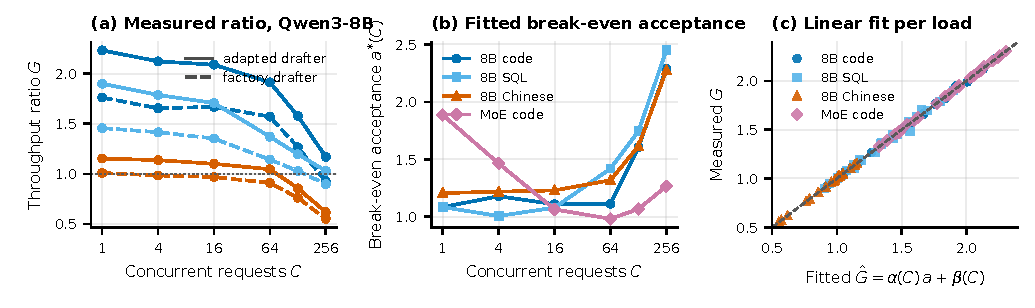
\includegraphics[width=\linewidth]{figures/fig3_frontier.pdf}
\caption{Profitability frontier. (a) Measured speculative over plain throughput for factory (dashed) and adapted (solid) Qwen3-8B drafters; colors as in (b). (b) Fitted break-even acceptance per load. (c) Linear fit versus measurement for all domains and loads.}
\label{fig:frontier}
\end{figure}

\paragraph{Output-length protocol.} Saturated throughput depends on how outputs end (Table~\ref{tab:protocol}). In a batch of 600 requests submitted at once, natural stopping mixes a long drain phase at low concurrency, where speculation is favourable; forcing every output to 256 tokens removes it, and the adapted code drafter then stays below plain decoding. The closed-loop evaluation uses natural stopping, as production traffic does.

\begin{table}[!htbp]
\caption{Code domain, Qwen3-8B: speculative over plain throughput for 600 requests submitted at once, with natural stopping versus outputs forced to 256 tokens.}
\label{tab:protocol}
\centering\small
% generated by code/specsched/paper_assets.py -- do not edit by hand
\begin{tabular}{@{}lccc@{}}
\toprule
Drafter & Natural stop & Fixed 256 tokens & Difference\\
\midrule
N0 & 0.75$\times$ & 0.68$\times$ & $-0.06$ \\
N400 & 0.98$\times$ & 0.82$\times$ & $-0.16$ \\
N800 & 0.88$\times$ & 0.83$\times$ & $-0.06$ \\
N3200 & 1.02$\times$ & 0.85$\times$ & $-0.17$ \\
\bottomrule
\end{tabular}

\end{table}

\FloatBarrier
\section{Controller Details}\label{app:controller}

\begin{algorithm}[!htbp]
\caption{One control tick (every second).}
\label{alg:controller}
\begin{algorithmic}[1]
\STATE Read $C$, the queue, the speculative-decoding counters, TPOT, and the trainer's state; if more than 20 drafts were made in the last second, $\hat a\leftarrow0.7\,\hat a+0.3\,a_{\mathrm{1s}}$
\IF{the label $\ell$ changed}
\STATE reset the regime clock and $\hat a$, flush the trainer's buffer, restart the export schedule
\ENDIF
\IF{the trainer exported a new drafter}
\STATE hot-swap it; if speculation is off, enable it for 8\,s to measure the new drafter
\ENDIF
\IF{$\ell$ has no learning curve, or $\amax_\ell-\hat a\le0.02$, or the last swap raised $\hat a$ by less than 0.02}
\STATE $d\leftarrow0$
\ELSIF{$\Ghat_\ell(\amax_\ell,C)\le1$}
\STATE $d\leftarrow0$ \COMMENT{structural ceiling}
\ELSIF{TPOT $\le\Tslo$ and the server is not saturated}
\STATE $d\leftarrow$ largest $d\in\mathcal D$ with $T_0/(1-\kappa(C)d)\le0.9\,\Tslo$
\ELSE
\STATE $d\leftarrow\arg\max_{d\in\mathcal D,\,d\le0.5}V(d)$ of \cref{eq:value} if the maximum is positive, else $0$
\ENDIF
\IF{the requests learned in this regime reached the next export point}
\STATE request an export; the next export point doubles the gap (100, 200, 400, \dots)
\ENDIF
\STATE compute $z^{\star}$ by \cref{eq:switch}; switch to $z^{\star}$ if it has differed from $z$ for 3 ticks, the last switch is at least 10\,s old, and no probe is active
\end{algorithmic}
\end{algorithm}

\begin{table}[!htbp]
\caption{Constants of the controller, as fixed in the frozen checkpoint.}
\label{tab:constants}
\centering\small
\begin{tabular}{@{}ll@{}}
\toprule
Constant & Value\\
\midrule
Control period & 1\,s\\
SLO $\Tslo$ & $2\times$ single-request decode time (\nv{slo.m1}\,ms Qwen3-8B, \nv{slo.m2}\,ms MoE)\\
Duty levels $\mathcal D$ & $\{0, 0.1, 0.25, 0.5, 1\}$\\
Slack rule margin & predicted TPOT $\le0.9\,\Tslo$\\
Saturation & queue non-empty, or $C\ge0.95\times256$\\
Duty cap under saturation & 0.5\\
Training target $a^{\dagger}$ & $\hat a+0.8\,(\amax_\ell-\hat a)$\\
Data availability $\rho$ & arrivals plus buffered tokens spread over 10\,s\\
Horizon forecast $\widehat H$ & age of the regime, clipped to $[90,600]$\,s\\
Stop at ceiling & $\amax_\ell-\hat a\le0.02$\\
Stop on convergence & last swap raised $\hat a$ by $<0.02$ (measured $\ge8$\,s after the swap)\\
Speculation switch & 3 agreeing ticks, $\ge10$\,s between switches, 8\,s probe after a swap\\
Export schedule & after 100 requests in the regime, then doubling gaps; $\ge5$\,s between requests\\
Acceptance estimate & moving average with weight 0.3 on the last second (if $>20$ drafts)\\
\bottomrule
\end{tabular}
\end{table}

\FloatBarrier
\section{Policies}\label{app:policies}

\begin{table}[!htbp]
\caption{The eight policies of the frozen evaluation. All use the factory drafter at the start of each run.}
\label{tab:policies}
\centering\small
\begin{tabularx}{\linewidth}{@{}l>{\raggedright\arraybackslash}X>{\raggedright\arraybackslash}X>{\raggedright\arraybackslash}X@{}}
\toprule
Policy & Speculation & Training & Information used\\
\midrule
\pol{Production} & always on & none & none (no export, no memory reserve)\\
\pol{Static} & always on & none & none\\
\pol{Plain} & no drafter loaded & none & none\\
\pol{Switch} & \cref{eq:switch} & none & label, frontier\\
\pol{Threshold} & off whenever saturated & duty 0.5 whenever TPOT is within the SLO & load threshold\\
\pol{Always} & always on & duty 0.5 from the first request; swaps after 100, 200, 400, \dots{} requests & none\\
\pol{Informed} & always on & duty 0.5 from the start of phase B until 800 requests are learned; swaps at 100, 200, 400, 800 & start of phase B; stopping point chosen from the learning curves\\
\pol{Full} & \cref{eq:switch} & \cref{sec:method} & label, frontier, learning curve\\
\bottomrule
\end{tabularx}
\end{table}

\FloatBarrier
\section{Additional Results}\label{app:extra}

\begin{table}[!htbp]
\caption{Phase-B throughput (tok/s) of every run, the mean, and the coefficient of variation (CV) over the three repetitions.}
\label{tab:runs}
\centering\small
% generated by code/specsched/paper_assets.py -- do not edit by hand
\begin{tabular}{@{}lrrrrr@{}}
\toprule
Policy & Run 1 & Run 2 & Run 3 & Mean & CV\\
\midrule
\multicolumn{6}{@{}l}{\textit{8B code}}\\
Production speculation & 14{,}590 & 14{,}672 & 14{,}541 & 14{,}601 & 0.5\% \\
Static speculation & 14{,}392 & 14{,}229 & 14{,}224 & 14{,}282 & 0.7\% \\
Plain decoding & 16{,}851 & 16{,}861 & 16{,}896 & 16{,}869 & 0.1\% \\
Switch only & 16{,}537 & 15{,}660 & 15{,}651 & 15{,}949 & 3.2\% \\
Threshold rule & 15{,}141 & 16{,}330 & 16{,}450 & 15{,}974 & 4.5\% \\
Always train & 14{,}417 & 14{,}724 & 14{,}709 & 14{,}617 & 1.2\% \\
Informed schedule & 17{,}247 & 17{,}096 & 16{,}963 & 17{,}102 & 0.8\% \\
Full controller & 16{,}831 & 16{,}674 & 17{,}054 & 16{,}853 & 1.1\% \\
\multicolumn{6}{@{}l}{\textit{8B Chinese}}\\
Production speculation & 8{,}675 & 8{,}677 & 8{,}694 & 8{,}682 & 0.1\% \\
Static speculation & 8{,}494 & 8{,}594 & 8{,}491 & 8{,}526 & 0.7\% \\
Plain decoding & 16{,}795 & 16{,}793 & 16{,}793 & 16{,}794 & 0.0\% \\
Switch only & 16{,}149 & 15{,}722 & 16{,}414 & 16{,}095 & 2.2\% \\
Threshold rule & 15{,}928 & 15{,}639 & 13{,}782 & 15{,}116 & 7.7\% \\
Always train & 8{,}406 & 8{,}432 & 8{,}442 & 8{,}427 & 0.2\% \\
Informed schedule & 9{,}691 & 9{,}781 & 9{,}624 & 9{,}699 & 0.8\% \\
Full controller & 16{,}214 & 15{,}301 & 16{,}475 & 15{,}997 & 3.9\% \\
\multicolumn{6}{@{}l}{\textit{MoE code}}\\
Production speculation & 13{,}990 & 13{,}986 & 14{,}000 & 13{,}992 & 0.0\% \\
Static speculation & 13{,}847 & 13{,}861 & 13{,}870 & 13{,}859 & 0.1\% \\
Plain decoding & 7{,}472 & 7{,}466 & 7{,}458 & 7{,}465 & 0.1\% \\
Switch only & 13{,}839 & 13{,}770 & 13{,}841 & 13{,}816 & 0.3\% \\
Threshold rule & 7{,}486 & 7{,}485 & 7{,}496 & 7{,}489 & 0.1\% \\
Always train & 13{,}372 & 13{,}324 & 13{,}396 & 13{,}364 & 0.3\% \\
Informed schedule & 15{,}217 & 15{,}183 & 15{,}054 & 15{,}151 & 0.6\% \\
Full controller & 14{,}965 & 15{,}018 & 14{,}920 & 14{,}967 & 0.3\% \\
\bottomrule
\end{tabular}

\end{table}

\begin{table}[!htbp]
\caption{Per-run behaviour of \pol{Full} during phase B, and the node each run used.}
\label{tab:fullruns}
\centering\small
% generated by code/specsched/paper_assets.py -- do not edit by hand
\begin{tabular}{@{}lcrrcccrl@{}}
\toprule
Scenario & Run & B tok/s & Spec.\ on & Duty & Swaps & Final acc. & Train tok.\ (M) & Node\\
\midrule
8B code & 1 & 16{,}831 & 100\% & 0.079 & 3 & 2.65 & 0.74 & c0803 \\
8B code & 2 & 16{,}674 & 100\% & 0.074 & 3 & 2.67 & 0.67 & c0806 \\
8B code & 3 & 17{,}054 & 100\% & 0.050 & 3 & 2.67 & 0.50 & c0806 \\
8B Chinese & 1 & 16{,}214 & 2\% & 0.018 & 1 & 1.20 & 0.39 & c0803 \\
8B Chinese & 2 & 15{,}301 & 2\% & 0.013 & 1 & 1.18 & 0.36 & c0803 \\
8B Chinese & 3 & 16{,}475 & 1\% & 0.017 & 1 & 1.17 & 0.39 & c0812 \\
MoE code & 1 & 14{,}965 & 100\% & 0.075 & 4 & 2.97 & 0.71 & c0813 \\
MoE code & 2 & 15{,}018 & 100\% & 0.079 & 4 & 2.99 & 0.72 & c0812 \\
MoE code & 3 & 14{,}920 & 100\% & 0.098 & 4 & 2.97 & 0.99 & c0803 \\
\bottomrule
\end{tabular}

\end{table}

\begin{table}[!htbp]
\caption{TPOT in milliseconds (means over three runs): median in the light chat phases A1 and A2, and 99th percentile in the saturated phase B.}
\label{tab:latency}
\centering\small
% generated by code/specsched/paper_assets.py -- do not edit by hand
\begin{tabular}{@{}lccccccccc@{}}
\toprule
& \multicolumn{3}{c}{8B code} & \multicolumn{3}{c}{8B Chinese} & \multicolumn{3}{c}{MoE code}\\
\cmidrule(lr){2-4}\cmidrule(lr){5-7}\cmidrule(l){8-10}
Policy & A1 p50 & B p99 & A2 p50 & A1 p50 & B p99 & A2 p50 & A1 p50 & B p99 & A2 p50\\
\midrule
Static speculation & 5.77 & 22.01 & 5.66 & 5.70 & 36.54 & 5.69 & 11.17 & 23.42 & 11.09 \\
Plain decoding & 8.92 & 15.08 & 8.92 & 8.92 & 15.35 & 8.86 & 16.61 & 33.83 & 16.53 \\
Switch only & 5.69 & 17.27 & 5.65 & 5.70 & 18.84 & 5.73 & 11.13 & 23.52 & 11.11 \\
Informed schedule & 5.77 & 22.88 & 4.74 & 5.77 & 37.41 & 5.06 & 11.28 & 22.69 & 10.19 \\
\rowcolor{resultgraylight}Full controller & 6.35 & 20.88 & 5.56 & 6.36 & 18.44 & 5.85 & 11.07 & 22.58 & 10.04 \\
\bottomrule
\end{tabular}

\end{table}

\begin{table}[!htbp]
\caption{Costs of the mechanisms, measured inside the frozen runs.}
\label{tab:mechanisms}
\centering\small
% generated by code/specsched/paper_assets.py -- do not edit by hand
\begin{tabularx}{\linewidth}{@{}>{\raggedright\arraybackslash}p{0.27\linewidth}>{\raggedright\arraybackslash}p{0.33\linewidth}>{\raggedright\arraybackslash}X@{}}
\toprule
Mechanism & Measurement & Result\\
\midrule
Feature export + trainer memory reserve & Production vs.\ static speculation, saturated throughput & 8B code 2.2\%, 8B Chinese 1.8\%, MoE code 1.0\% \\
Runtime-off state vs.\ no drafter & Switch only vs.\ plain decoding, saturated throughput & 8B code $-4.4$\%, 8B Chinese $-3.1$\% \\
Drafter hot swap (8B) & 181 swaps in the frozen runs & median 0.71\,s, range 0.33--1.58\,s \\
Drafter hot swap (MoE) & 70 swaps in the frozen runs & median 0.31\,s, range 0.21--0.76\,s \\
Speculation switch & 74 switches, RPC round trip & median 22\,ms, max.\ 66\,ms \\
Training data used (full controller) & Requests consumed by the trainer, of 16{,}400 served per run & 8B code 1{,}746 (11\%), 8B Chinese 849 (5\%), MoE code 2{,}648 (16\%) \\
\bottomrule
\end{tabularx}

\end{table}

\FloatBarrier
\section{Simulator and Held-out Validation}\label{app:sim}

\paragraph{Model.} The simulator (\texttt{sched/sim.py}) advances in 1\,s steps on one GPU. Arrivals of the current domain set the operating concurrency $C$ by solving $\Theta(C)=$ demand, where $\Theta$ includes the frontier gain when speculation is on and the factor $1-\kappa(C)\,d$ when the trainer runs; demand beyond the capacity at $C{=}256$ accumulates in a queue. TPOT is the step time divided by the frontier gain and by $1-\kappa(C)\,d$. Served requests feed a training buffer; training at duty $d$ consumes tokens at rate $r\,d$ and moves acceptance along the domain's learning curve, with the measured fraction transferring to chat. Goodput counts output tokens served in seconds whose TPOT and queueing delay meet the SLO. The simulator and the calibration file were frozen before the validation (hashes in \cref{tab:manifest}).

\paragraph{Workloads.} V1 replays BurstGPT \citep{wang2024burstgpt} chat logs on days 4, 6, 8, 12, 16, and 20 and API logs on days 15, 21, and 22 (development had used day 2 and day 10 only), each for 24\,h and scaled so that the 95th-percentile demand is 0.6, 0.8, or 1.0 times capacity, and the Azure 2023 chat and code traces \citep{patel2024splitwise} for one hour at scales 0.6--1.2. V2 draws 60 bursts: a chat, code, or function-calling phase, followed by a code, SQL, or function-calling burst at 1.0, 1.05, or 1.2 times capacity lasting 5, 10, 20, 60, 180, or 600\,s, and a recovery phase. V3 draws 40 regimes in which traffic switches to Chinese at 128--256 concurrent requests or 1.1 times capacity for 600--1{,}800\,s. V4 draws 20 scenarios with a calm phase of 120--900\,s, a moderate phase, and a 600\,s surge, each at seven surge levels from 0.9 to 1.2 times capacity.

\begin{table}[!htbp]
\caption{Pre-declared criteria of the frozen-simulator validation and their outcomes.}
\label{tab:heldout}
\centering\small
% generated by code/specsched/paper_assets.py -- do not edit by hand
\begin{tabularx}{\linewidth}{@{}l>{\raggedright\arraybackslash}p{0.13\linewidth}>{\raggedright\arraybackslash}X>{\raggedright\arraybackslash}X>{\raggedright\arraybackslash}p{0.19\linewidth}@{}}
\toprule
& Scenarios & Pre-declared criterion & Outcome & Verdict\\
\midrule
V1 & 35 unseen trace windows & Goodput $\ge 0.97\times$ the best simple policy; training tokens $\le 10\%$ of idle-time training (OSD) & Goodput: 35/35 (min.\ 0.994, median 1.006, best in 25); training: 31/35 & Goodput met; training criterion failed where OSD itself barely trains \\
V2 & 60 random bursts & Not below speculation-always in $\ge 80\%$ of bursts lasting $\ge 10$\,s & 45/49 (91.8\%); worst loss 1.4\% & Met; strict wins only from 60\,s, reliable from 180\,s \\
V3 & 40 Chinese (ceiling) regimes & Above speculation-always and both reactive training policies; ratio $\ge 1.5\times$ & Ordering 40/40; ratio 1.41--2.00$\times$ at feasible saturation, min.\ 1.12$\times$ under overload & Ordering met; magnitude criterion failed \\
V4 & 20 surge scenarios & Max.\ violation-free surge $\ge$ OSD and $\ge$ AccDrop in $\ge 80\%$ & 19/20; mean surge 1.12 vs AccDrop 1.13, OSD 1.08 & Met; no advantage over AccDrop \\
\bottomrule
\end{tabularx}

\end{table}

\begin{table}[!htbp]
\caption{V2 by burst length: goodput of the controller relative to \pol{SpecAlways}.}
\label{tab:duration}
\centering\small
% generated by code/specsched/paper_assets.py -- do not edit by hand
\begin{tabular}{@{}rrrrrrr@{}}
\toprule
Burst (s) & Cases & Strict wins & Ties & Losses & Median ratio & Max.\ ratio\\
\midrule
5 & 11 & 45\% & 45\% & 9\% & 1.000 & 1.05 \\
10 & 8 & 38\% & 50\% & 12\% & 1.000 & 1.01 \\
20 & 10 & 30\% & 50\% & 20\% & 1.000 & 1.13 \\
60 & 8 & 62\% & 25\% & 12\% & 1.056 & 1.31 \\
180 & 12 & 92\% & 8\% & 0\% & 1.294 & 8.39 \\
600 & 11 & 82\% & 18\% & 0\% & 7.044 & 28.43 \\
\bottomrule
\end{tabular}

\end{table}


\end{document}
